\graphicspath{{images/}}
\renewcommand{\theequation}{\arabic{chapter}.\arabic{equation}}

\chapter{MARCO METODOLÓGICO}

Este capítulo describe el método completo, organizado en las cuatro
unidades de la arquitectura. Comienza por la construcción del entorno
de simulación (U1), con dos caminos posibles: la importación de una
intersección real desde OpenStreetMap, prevista para el cruce de Lima,
y la descripción directa de nodos y vías, que es la que se usó para los
escenarios evaluados en esta fase. Sigue con la formulación e
implementación del agente de aprendizaje por refuerzo (U2), la
instrumentación de las métricas (U3) y el plan de pruebas con el que se
obtienen los resultados del Capítulo~\ref{cap:resultados}. La
coordinación distribuida entre semáforos vecinos (U4), formulada en el
Capítulo~I, se implementa en la Sección~\ref{sec:u4} sobre los
escenarios de varios semáforos.

\section{Alcance y unidades}

\noindent\textbf{U1: Preprocesamiento.} Comprende todas las tareas
relacionadas con la construcción del escenario: la instalación y
configuración de SUMO, la obtención de la red (por conversión de un
recorte de OSM o por descripción directa de nodos y vías), la
definición de la demanda vehicular y la creación de archivos de
configuración reproducibles (\texttt{.net.xml} para la red,
\texttt{.rou.xml} para la demanda y \texttt{.sumocfg} para el
escenario). El resultado de U1 es un escenario listo para simular.

\noindent\textbf{U2: Entrenamiento.} Toma como entrada el escenario de
U1 y ejecuta SUMO a través de la interfaz TraCI para que un agente de
aprendizaje por refuerzo observe el estado del tráfico y modifique
las fases de los semáforos.  En U2 no se modifican la red ni las
rutas: el enfoque se centra en el algoritmo de control.

\noindent\textbf{U3: Medición.} Calcula, sobre las mismas salidas de
SUMO y para todos los controles comparados, las métricas de desempeño
con las que se evalúa el sistema (Sección~\ref{sec:u3}).

\noindent\textbf{U4: Coordinación distribuida.} Añade mensajería entre
agentes vecinos, estado extendido, penalización por \textit{spillback}
y un algoritmo con aproximación de funciones (Sección~\ref{sec:u4}).
Se evalúa en variantes incrementales sobre los escenarios de varios
semáforos, frente a los mismos controles de referencia que U2, de modo
que el aporte de la comunicación quede aislado del resto de cambios.

\section{Requisitos de hardware}

Todas las corridas de esta fase (U1 a U4 y el plan de pruebas) se
ejecutaron en el equipo de la Tabla~\ref{tab:hw}, un computador de
escritorio sin GPU. Ningún modelo la necesita: las redes de IPPO, DQN
y MAPPO tienen dos capas ocultas de 64 unidades, y el costo lo domina
la simulación en SUMO, no la red. Cada entrenamiento usa un solo hilo y
la cola de trabajos del plan de pruebas corre hasta 11 a la vez. Con la
máquina así cargada, un episodio de una hora simulada tarda, en
mediana, entre 5 y 17~s en los escenarios de dos y tres semáforos y
entre 24 y 31~s en la malla de nueve; un entrenamiento completo
(200 episodios más sus validaciones) toma entre 21 minutos y 1.9~horas
según el escenario y el modelo (Tabla~\ref{tab:plan2-costo}).

\begin{table}[H]
\setstretch{1}
\centering
\footnotesize
\begin{tabular}{p{3.2cm}p{9.2cm}}
\toprule
Componente & Equipo usado \\
\midrule
CPU & AMD Ryzen 7 3700X, 8 núcleos y 16 hilos \\
RAM & 16~GB \\
GPU & no se usa; PyTorch 2.14.0 en su versión para CPU \\
Almacenamiento & SSD NVMe de 1~TB \\
Sistema operativo & Windows 10 Pro \\
Software & SUMO 1.25.0; Python 3.14 con \texttt{traci}, \texttt{sumolib}, NumPy 2.5.1, SciPy 1.18.0, Matplotlib 3.11.0 y PyTorch 2.14.0+cpu \\
Paralelismo & un hilo por entrenamiento; hasta 11 procesos a la vez \\
\bottomrule
\end{tabular}
\caption{Equipo en el que se ejecutaron todas las corridas.}
\label{tab:hw}
\end{table}
% fuente: Win32_Processor, Win32_ComputerSystem y Get-PhysicalDisk (24.09.2026);
% python -c "import torch, numpy, scipy, matplotlib" (versiones); plan2/cola.py (--cpus 11)

\section{Instalación y configuración de SUMO}

\begin{enumerate}
  \item \textbf{Descargar e instalar SUMO.} Obtenga la versión estable
    de SUMO desde el sitio oficial y siga las instrucciones de
    instalación para su sistema operativo.  SUMO incluye varios
    ejecutables de consola, como \emph{sumo} (simulación),
    \emph{sumo-gui} (versión con interfaz gráfica) y
    \emph{netconvert} (importación de redes).
    Instale también Python~3, necesario para ejecutar los
    scripts auxiliares.

  \item \textbf{Configurar el entorno.} Defina la variable de
    entorno \verb|SUMO_HOME| apuntando al directorio donde se instaló
    SUMO y añada la carpeta \verb|bin| al \verb|PATH| del sistema.
    Esto permite invocar los programas de SUMO desde cualquier
    terminal.

  \item \textbf{Verificar la instalación.} Abra una terminal y ejecute
    los siguientes comandos.  Deben devolver la versión instalada de
    SUMO para confirmar que el entorno está listo:

    {\footnotesize\begin{verbatim}
sumo -V
sumo-gui -V
    \end{verbatim}
    }
\end{enumerate}

%----------------------------------------------------------------------
\section{Limpieza y configuración del escenario OSM \texorpdfstring{$\rightarrow$}{a} SUMO}
\label{sec:osm-limpieza}

Cuando la red proviene de cartografía real, es necesario revisar y
ajustar el escenario para que represente fielmente la intersección de
estudio y resulte adecuado para el entrenamiento del agente de control.
Este proceso consiste en eliminar elementos irrelevantes, corregir
inconsistencias topológicas y configurar adecuadamente los semáforos y
la demanda. El procedimiento que sigue es el previsto para el cruce
real de Lima; los cinco escenarios evaluados en esta fase se
construyeron por el camino alternativo descrito en la
Sección~\ref{sec:escenarios}, escribiendo directamente los archivos de
nodos y vías, por lo que no requirieron limpieza. Las figuras de esta
sección ilustran el procedimiento sobre una intersección de ejemplo y
no corresponden a ninguno de los escenarios evaluados.

\subsection*{Eliminación y simplificación de la red}

\begin{enumerate}
  \item \textbf{Abrir la red en un editor.} Utilice \verb|sumo-gui| o
    \texttt{netedit}, las herramientas de SUMO destinadas a la
    inspección y edición de redes. Desde la interfaz gráfica se puede
    seleccionar manualmente cada calle, carril e intersección para
    examinar su geometría y atributos.

  \item \textbf{Eliminar calles irrelevantes.} Desactive o borre los
    segmentos de vía que no formen parte del cruce objeto de estudio.
    En \texttt{netedit} esto puede realizarse en modo ``Edge''
    seleccionando los elementos y pulsando la tecla Suprimir. También
    se pueden modificar jerarquías de carreteras para mantener
    únicamente arterias principales y desechar caminos secundarios.

  \item \textbf{Ajustar sentidos de circulación.} Verifique que las
    direcciones de cada carril coinciden con la realidad (por ejemplo,
    si un carril debería ser unidireccional). En \texttt{netedit}
    es posible invertir la dirección de un carril o fusionar dos
    carriles paralelos empleando la herramienta de edición de lanes.

  \item \textbf{Simplificar nodos complejos.} Algunas importaciones
    desde OSM generan nodos excesivamente subdivididos. Estos pueden
    fusionarse mediante la opción de simplificación de intersecciones
    en \texttt{netconvert} o mediante edición manual. Una red más
    simple facilita el entrenamiento y reduce tiempos de simulación.
\end{enumerate}

Tras completar estos pasos, la red se limpia y simplifica. La
Figura~\ref{fig:netedit-before-after} muestra un ejemplo antes y
después de la limpieza realizada en \texttt{netedit} para el cruce
estudiado. Se observa cómo se eliminan calles secundarias y se ajusta
la orientación de los carriles.

\begin{figure}[H]
  \centering
  \subfigure[Vista inicial en \texttt{netedit} con la intersección
    importada; hay calles secundarias y direcciones de carril
    incorrectas.]{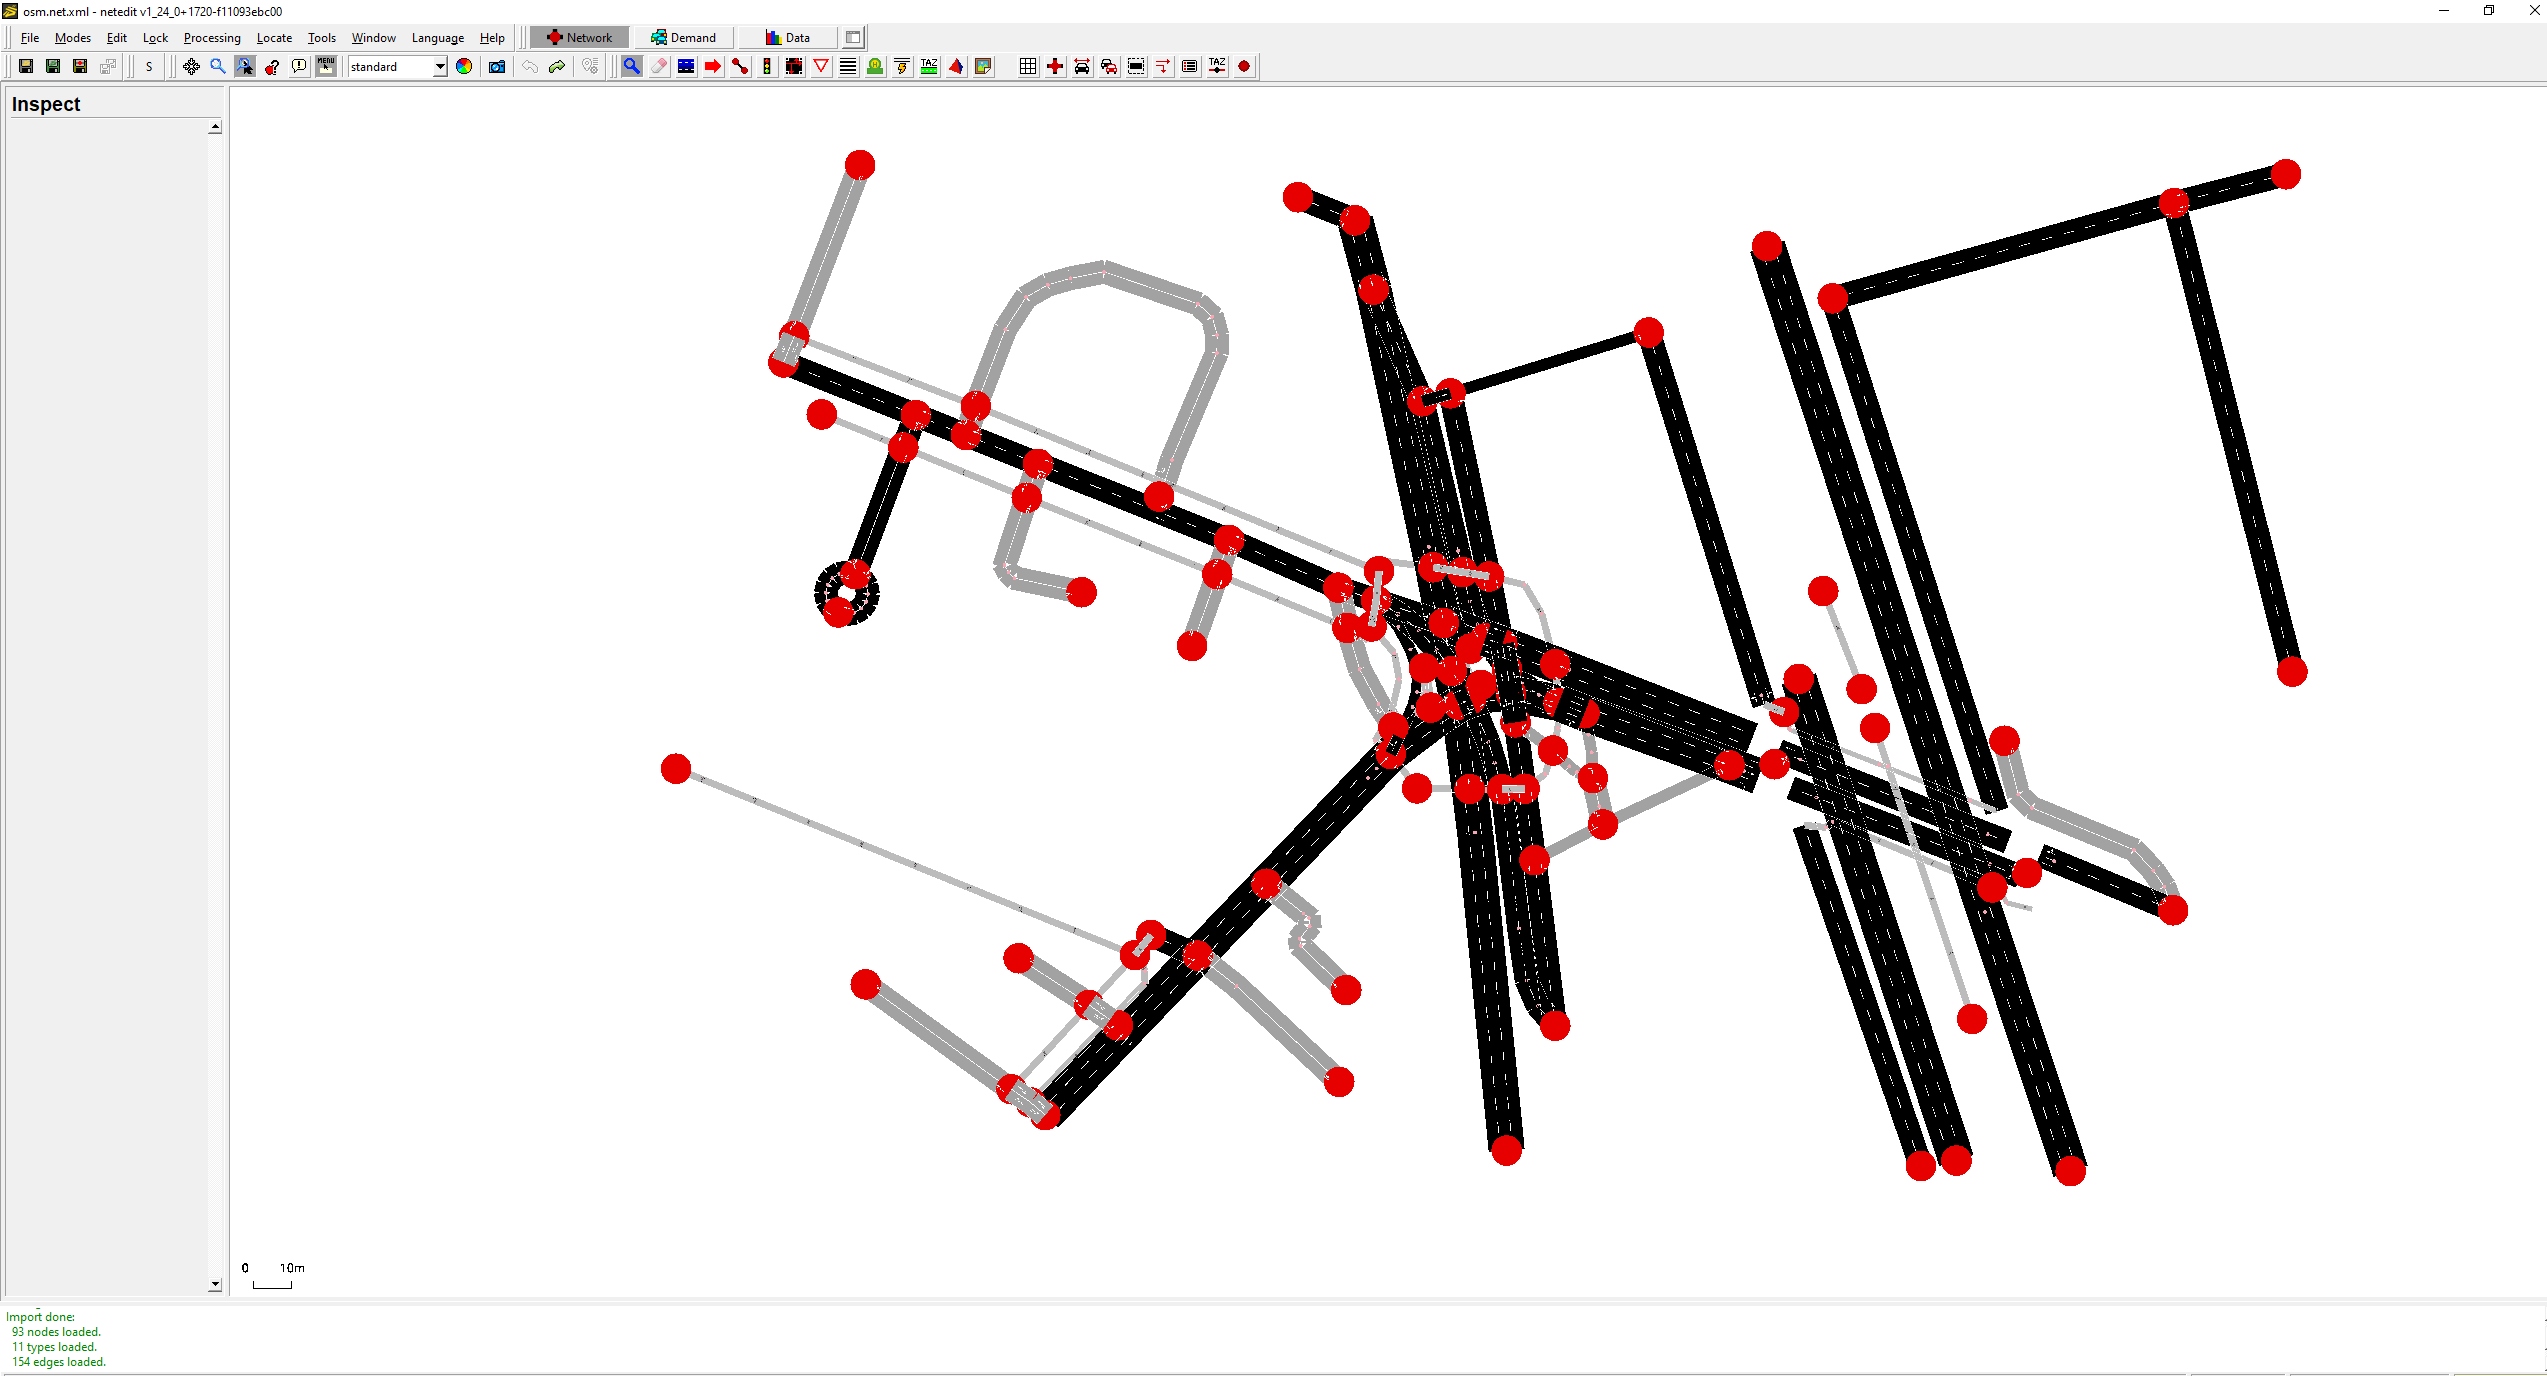
\includegraphics[width=0.48\textwidth]{NETEDIT.PNG}}
  \hfill
  \subfigure[Misma intersección tras la limpieza: calles irrelevantes
    eliminadas y sentidos de los carriles corregidos.]{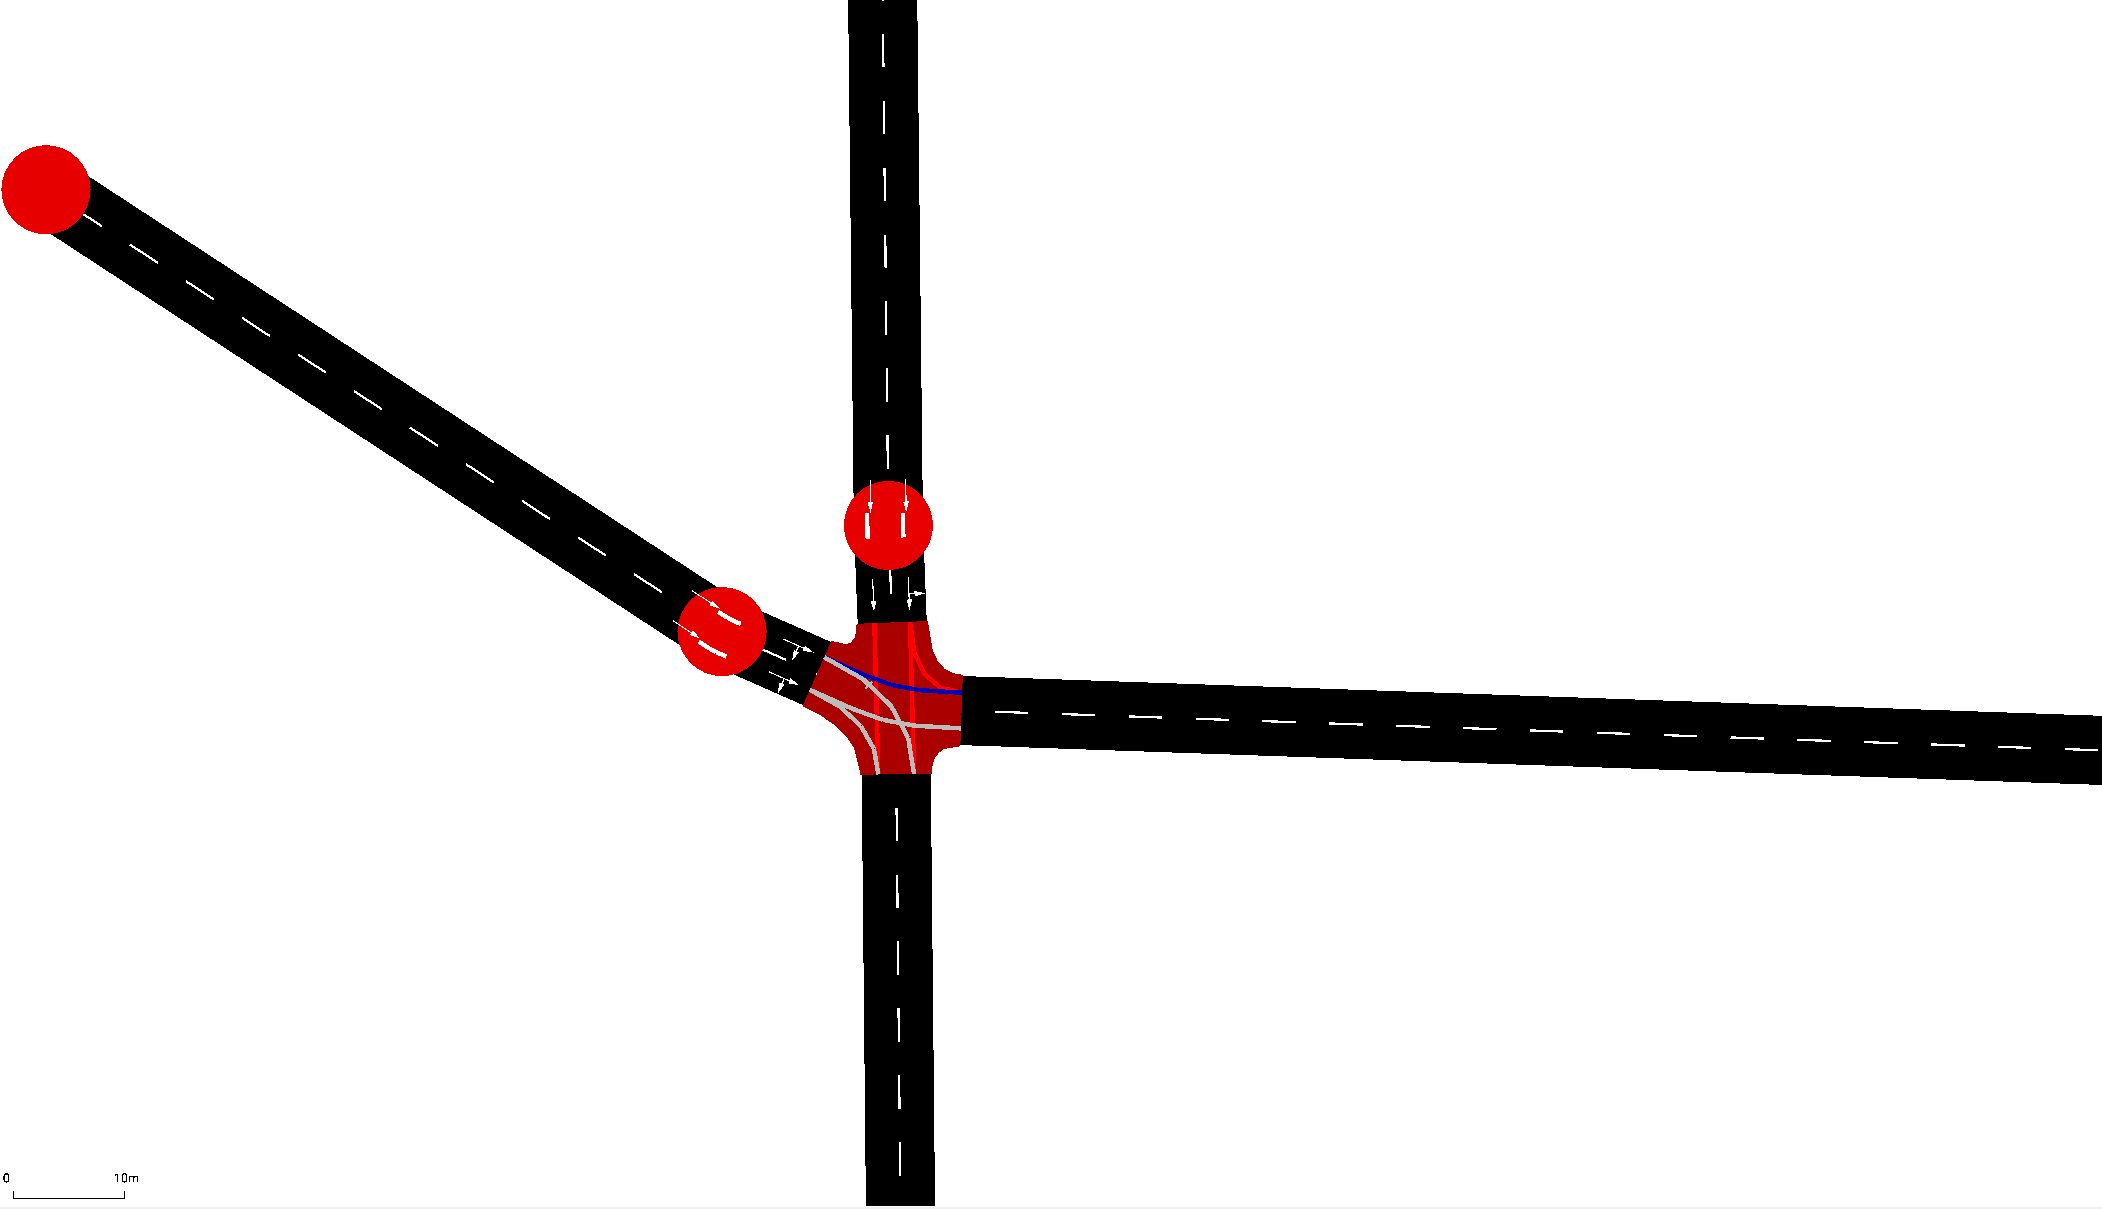
\includegraphics[width=0.48\textwidth]{conexiones.PNG}}
  \caption{Antes y después de la limpieza de la red en \texttt{netedit}, sobre una intersección de ejemplo importada desde OSM. Ilustra el procedimiento previsto para el cruce real de Lima; los escenarios evaluados en el Capítulo~\ref{cap:resultados} no provienen de OSM.}
  \label{fig:netedit-before-after}
\end{figure}

\subsection*{Configuración de semáforos y demanda}

\begin{enumerate}
  \item \textbf{Revisar semáforos importados.} Si al generar el
    escenario se activó la opción ``Traffic lights'', los semáforos
    aparecerán como nodos \verb|<tlLogic>| en el archivo
    \texttt{.net.xml}. Utilice \emph{sumo-gui} o \texttt{netedit}
    para inspeccionar las fases (colores) y tiempos asignados
    automáticamente. Ajuste los valores para que respeten las
    normativas locales: el ámbar suele fijarse entre 3 y 4~s según la
    velocidad de aproximación, y las duraciones de verde deben ser
    proporcionales al flujo de cada aproximación. Los escenarios de
    esta tesis usan el ámbar de 3~s que \texttt{netconvert} asigna por
    omisión, valor que se mantiene idéntico en todos los controles
    comparados.

  \item \textbf{Crear o modificar programas de semáforos.} Para
    controlar manualmente los semáforos se puede definir un archivo
    adicional \texttt{.add.xml}. Un ejemplo sencillo de un programa
    estático para una intersección de dos fases es:

{\footnotesize\begin{verbatim}
<additional>
  <tlLogic id="semaforo_C" type="static" programID="fijo" offset="0">
    <!-- Fase 0: verde en el eje N-S -->
    <phase duration="25" state="GGgrrrGGgrrr"/>
    <!-- Fase 1: ambar en el eje N-S -->
    <phase duration="3"  state="yyyrrryyyrrr"/>
    <!-- Fase 2: verde en el eje E-O -->
    <phase duration="25" state="rrrGGgrrrGGg"/>
    <!-- Fase 3: ambar en el eje E-O -->
    <phase duration="3"  state="rrryyyrrryyy"/>
  </tlLogic>
</additional>
\end{verbatim}
}

    El atributo \texttt{state} lleva un carácter por cada movimiento
    permitido en la intersección, en el orden en que los numera el
    archivo de red: \texttt{G} y \texttt{g} para verde con y sin
    prioridad, \texttt{y} para ámbar y \texttt{r} para rojo. El ejemplo
    corresponde al escenario de cruce simple descrito en la
    Sección~\ref{sec:escenarios}, con doce movimientos. El atributo
    \texttt{offset} desplaza el inicio del ciclo y es lo que permite
    coordinar intersecciones sucesivas en una onda verde.

    Este archivo debe referenciarse en el fichero \texttt{.sumocfg}
    dentro del apartado \verb|<additional-files>| para que SUMO lo
    cargue junto con la red y las rutas. Si se decide mantener los
    semáforos generados automáticamente, conviene al menos fijar sus
    tiempos mínimos y comprobar que las fases son coherentes.

  \item \textbf{Configurar la demanda.} La demanda se define en el
    archivo \texttt{.rou.xml} mediante elementos \verb|<flow>|, cada
    uno con su origen y destino, su periodo de vigencia y su tasa de
    llegada. Un ejemplo tomado del escenario de cruce simple es:

{\footnotesize\begin{verbatim}
<routes>
  <vType id="auto" accel="2.6" decel="4.5" sigma="0.5"
         length="5" minGap="2.5" maxSpeed="13.89"/>
  <!-- Periodo 1 (0-1800 s): punta en el eje Norte-Sur -->
  <flow id="p1_N_S" type="auto" from="N_C" to="C_S"
        begin="0" end="1800" vehsPerHour="650"/>
  <!-- Periodo 2 (1800-3600 s): la punta se invierte -->
  <flow id="p2_N_S" type="auto" from="N_C" to="C_S"
        begin="1800" end="3600" vehsPerHour="150"/>
</routes>
\end{verbatim}
}

    El atributo \verb|vehsPerHour| inserta los vehículos
    \emph{equiespaciados} en el tiempo, de modo que la secuencia de
    llegadas es la misma en todas las corridas y la semilla solo altera
    el comportamiento individual de los conductores. Para obtener
    llegadas aleatorias hay que usar \verb|period="exp(X)"|, que
    convierte la inserción en un proceso de Poisson. La elección entre
    ambas y sus consecuencias se discuten en la
    Sección~\ref{sec:plan}. El atributo \verb|sigma| del tipo de
    vehículo controla la imperfección del conductor y es, junto con el
    factor de velocidad individual, la única fuente de variabilidad
    entre semillas cuando las llegadas son equiespaciadas.

  \item \textbf{Actualizar los archivos de configuración.} Una vez
    depurada la red y configurados los semáforos y la demanda,
    asegúrese de que el archivo de configuración \texttt{.sumocfg}
    referencia correctamente todos los ficheros relevantes:
    \texttt{.net.xml}, \texttt{.rou.xml} y, en su caso,
    \texttt{.add.xml}. Ejecute una simulación breve para verificar
    que el escenario se carga sin mensajes de error.
\end{enumerate}

\subsection*{Herramientas útiles}

Para tareas de limpieza y configuración puede emplear las siguientes
herramientas que acompañan a SUMO:

\begin{itemize}
  \item \textbf{netconvert:} conversor de redes. Genera el
    \texttt{.net.xml} a partir de un recorte de OSM o de archivos de
    nodos, vías y conexiones escritos a mano, y es también donde se
    fijan los tiempos por omisión de los semáforos generados
    (\verb|--tls.green.time|, \verb|--tls.left-green.time|).
  \item \textbf{netedit:} editor gráfico que permite crear, modificar
    y depurar redes, así como editar semáforos, conexiones y
    restricciones de circulación. Resulta idóneo para eliminar
    segmentos irrelevantes y ajustar sentidos de vía tras una
    importación desde OSM.
  \item \textbf{sumo-gui:} interfaz gráfica de simulación que permite
    visualizar el comportamiento de los vehículos y los semáforos en
    tiempo real. Es útil para validar la red depurada y detectar
    cuellos de botella o comportamientos anómalos.
\end{itemize}

\section{Importación de un cruce desde OSM}

Para llevar al \textit{pipeline} una intersección real, el primer paso
es importar su cartografía. SUMO ofrece dos vías: el asistente gráfico
\emph{osmWebWizard}, que se describe a continuación, y la descarga
manual del recorte con \verb|osmGet.py| seguida de su conversión con
\verb|netconvert|, que da control más fino sobre los filtros de
importación a cambio de más pasos. Ambas producen el mismo tipo de
archivo \texttt{.net.xml} y requieren después la limpieza de la
Sección~\ref{sec:osm-limpieza}. Este procedimiento es el previsto para
el cruce de Lima y no se aplicó a los escenarios evaluados en esta
fase.

\subsection{Asistente OSM (\emph{osmWebWizard})}

\begin{enumerate}
  \item Ejecute el script \verb|osmWebWizard.py| desde la carpeta de
    herramientas de SUMO.  El script abre un navegador donde se puede
    navegar sobre el mapa de OSM, seleccionar la zona deseada y
    generar el escenario automáticamente.  El uso básico es:
    {\footnotesize\begin{verbatim}
python tools/osmWebWizard.py
    \end{verbatim}
    }

  \item Seleccione ``Lima, Peru'' en el buscador y ajuste el
    \emph{bounding box} sobre la intersección de interés.  Active la
    opción “Traffic lights” si desea que se importen los semáforos y
    pulse “Generate Scenario”.  El asistente creará la red
    \texttt{.net.xml}, una demanda aleatoria y un fichero
    \texttt{.sumocfg}; además iniciará \emph{sumo-gui} con el
    escenario resultante.  Los archivos se guardan en un
    subdirectorio con marca temporal.

  \item Revise la red en \emph{sumo-gui} y, si detecta calles
    desconectadas o giros imposibles, ajuste el recorte y repita la
    generación hasta obtener una red consistente.
\end{enumerate}

Para ilustrar este proceso, la Figura~\ref{fig:import-osm-sumo} muestra
la selección del área en OSM y la red generada en SUMO. A la
izquierda se observa el recuadro delimitado sobre el mapa en el asistente
\emph{osmWebWizard}, y a la derecha la red importada tal como aparece en
\emph{sumo-gui}.

\begin{figure}[H]
  \centering
  \subfigure[Selección del \textit{bounding box} en OSM mediante el
    asistente \emph{osmWebWizard}.]{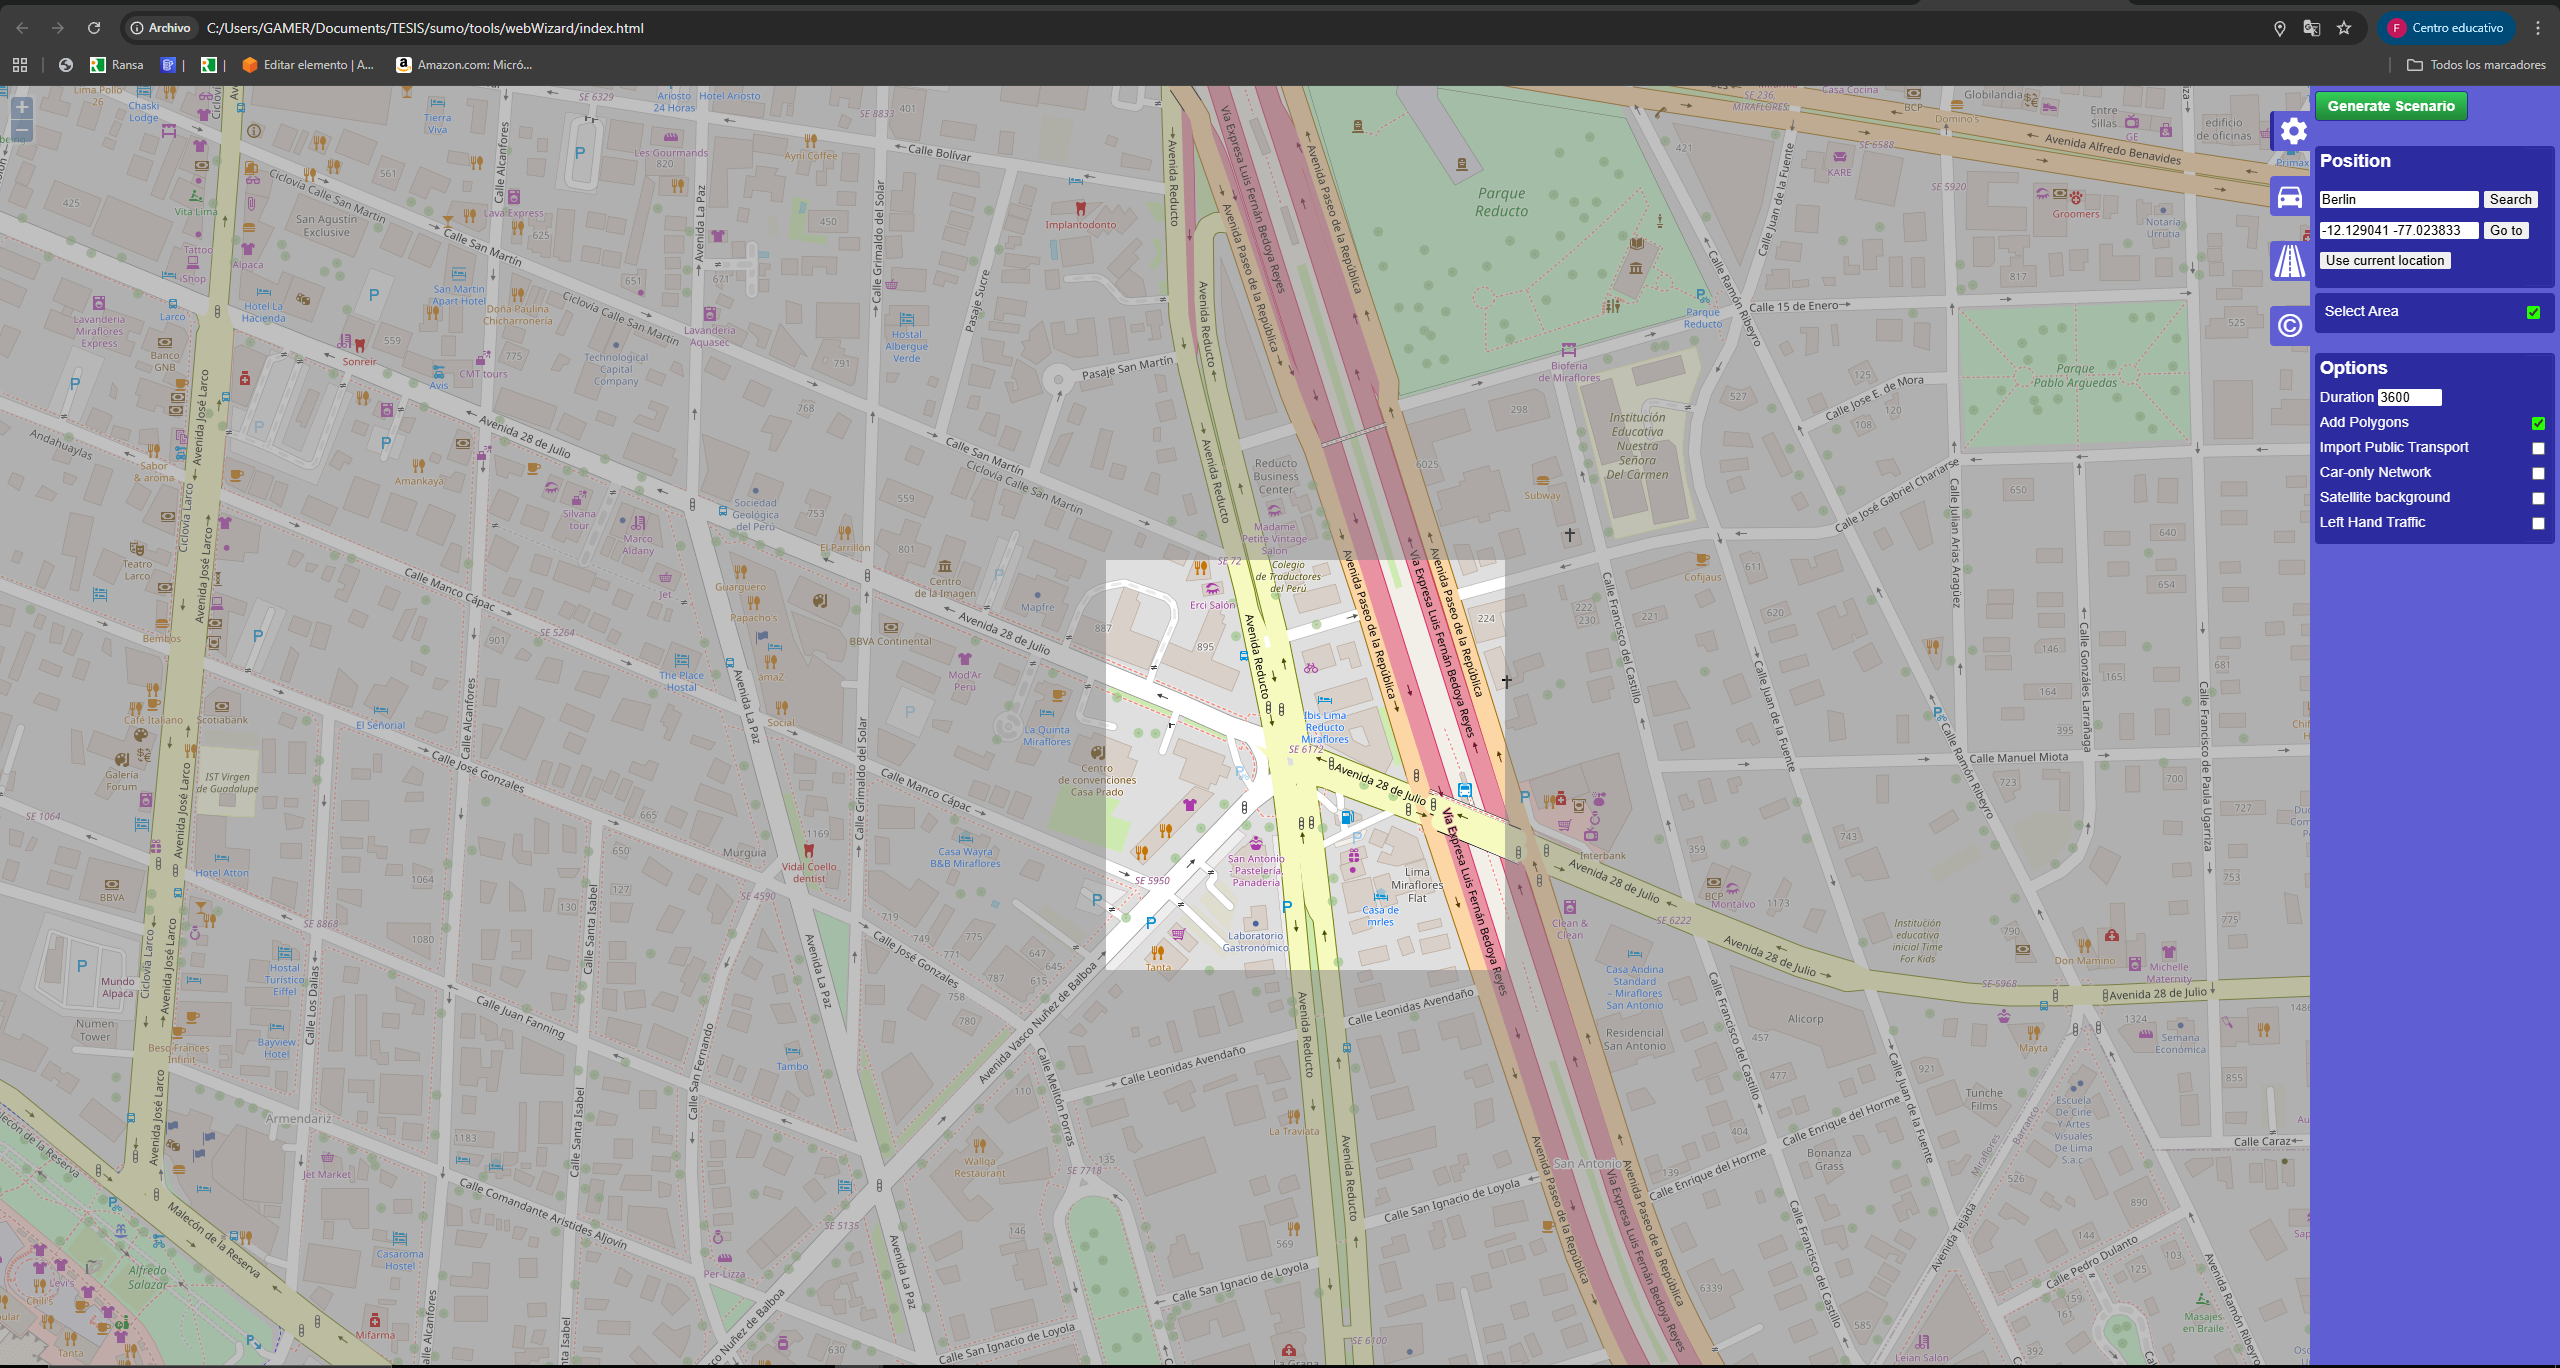
\includegraphics[width=0.48\textwidth]{OSM.PNG}}
  \hfill
  \subfigure[Red del cruce generada automáticamente en \emph{sumo-gui}.]{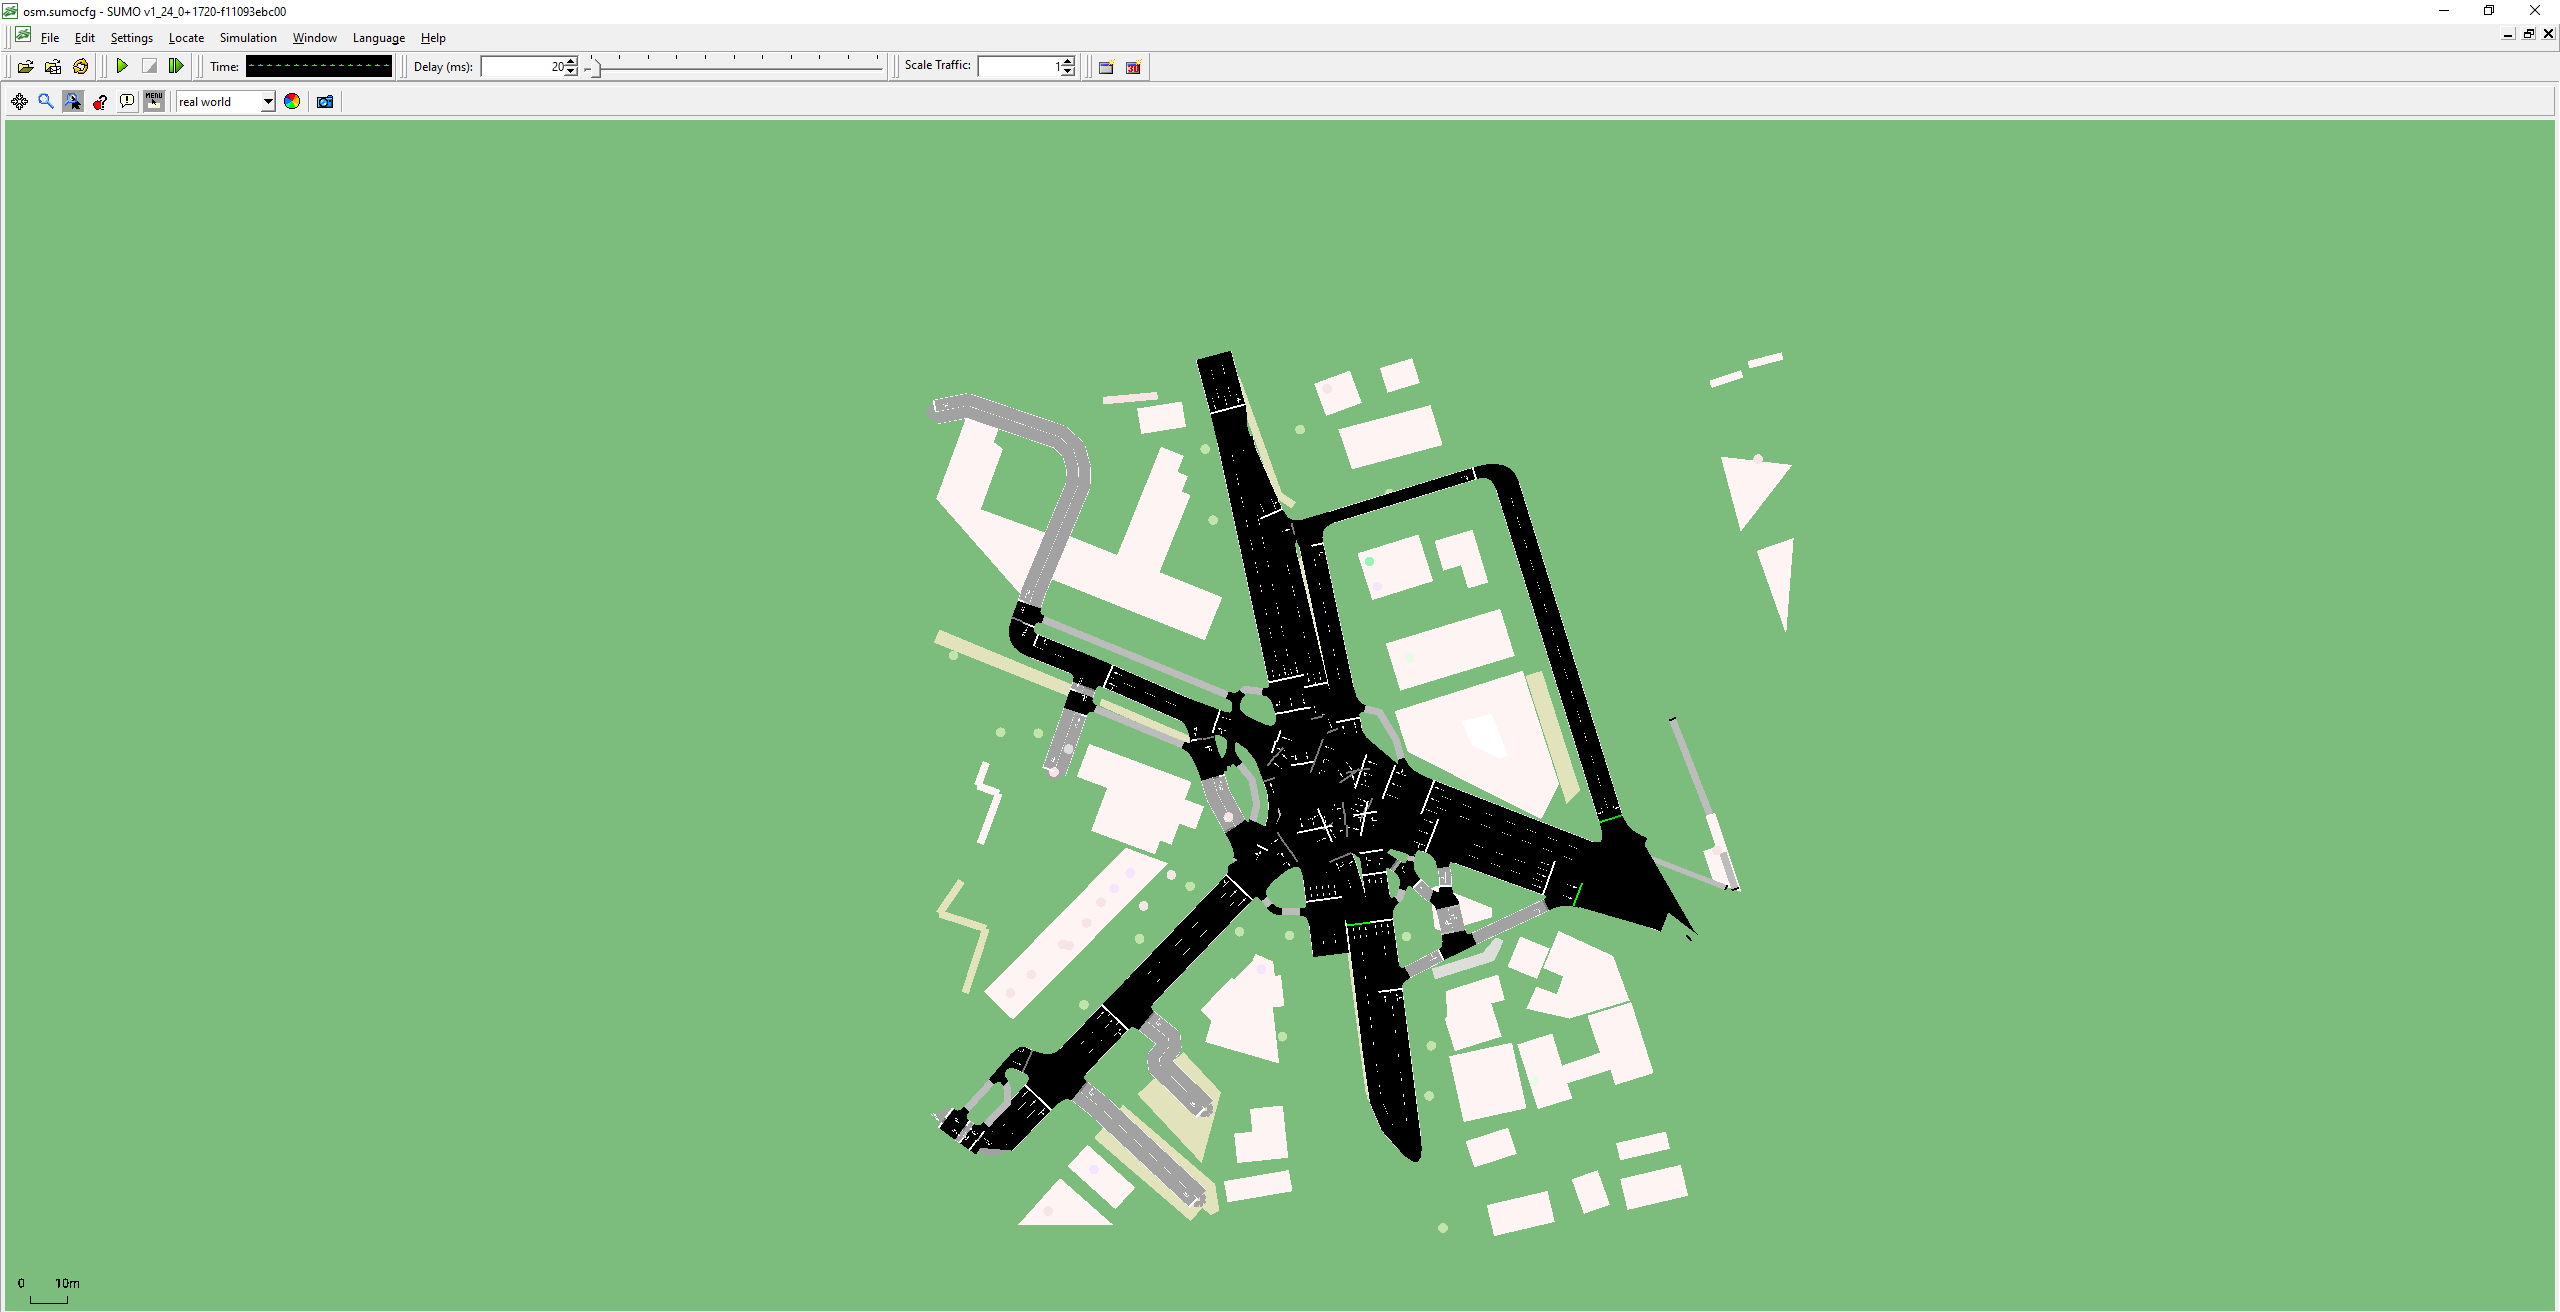
\includegraphics[width=0.48\textwidth]{SUMO.PNG}}
  \caption{Importación de un cruce desde OSM a SUMO mediante el asistente \emph{osmWebWizard}.}
  \label{fig:import-osm-sumo}
\end{figure}

\section{Generación y ejecución del escenario}

\subsection{Generar rutas de vehículos}

Con la red validada, se requieren rutas de vehículos para simular el
tráfico. Hay dos caminos:

\begin{enumerate}
  \item \textbf{Demanda declarada por flujos.} Es la que se usa en esta
    tesis: cada movimiento de la intersección se declara como un
    \verb|<flow>| con su origen, su destino, su periodo de vigencia y
    su tasa horaria, según el ejemplo de la
    Sección~\ref{sec:osm-limpieza}. SUMO calcula la ruta más corta
    entre origen y destino, de modo que no hace falta un paso previo de
    enrutamiento. Este camino da control explícito sobre el reparto
    direccional de la demanda, que es justamente lo que se manipula
    para construir los periodos de punta invertida.

  \item \textbf{Demanda aleatoria preliminar.} Cuando solo se necesita
    poblar una red recién importada para inspeccionarla, la
    herramienta \verb|randomTrips.py| de SUMO genera viajes entre pares
    de arcos elegidos al azar, con la intensidad que fija la opción
    \verb|-p| y una semilla reproducible con \verb|--seed|. Es útil
    para validar visualmente una red importada de OSM, pero no produce
    un reparto direccional controlado, por lo que no se emplea para los
    experimentos.
\end{enumerate}

\subsection{Crear el archivo de configuración}

Agrupe los archivos de red (\texttt{.net.xml}), rutas
(\texttt{.rou.xml}) y, si procede, el programa de semáforos
(\texttt{.add.xml}) en un único archivo de configuración
\texttt{.sumocfg}.  Este fichero referencia todos los elementos de
entrada y define los intervalos de simulación.

\subsection{Ejecución de SUMO}

\begin{enumerate}
  \item Para simular de forma interactiva, ejecute SUMO con
    interfaz gráfica:
    {\footnotesize\begin{verbatim}
sumo-gui -c escenario.sumocfg
    \end{verbatim}
    }

  \item Para simulaciones por lotes sin interfaz gráfica, utilice el
    ejecutable \verb|sumo|:
    {\footnotesize\begin{verbatim}
sumo -c escenario.sumocfg
    \end{verbatim}
    }
    Los ejecutables de SUMO son aplicaciones de consola; las opciones
    \verb|--net| y \verb|--route-files| permiten especificar
    directamente los archivos de red y rutas si no se usa un
    \texttt{.sumocfg}.
\end{enumerate}

\section{Escenarios sintéticos de prueba}
\label{sec:escenarios}

Mientras se completa la importación del cruce real de Lima, los
módulos U2, U3 y U4 se desarrollaron y validaron sobre siete escenarios
sintéticos, construidos con \texttt{netconvert} a partir de archivos de
nodos y vías escritos a mano, del más simple al más complejo
(Tabla~\ref{tab:escenarios}). Los cuatro primeros comparten el mismo
nivel de demanda; el quinto, corredor\_alta, es el escenario de estrés
del módulo U4 y se describe en la Sección~\ref{sec:u4}; los dos
últimos, red\_alta y malla3, son los casos P4 y P5 del plan de pruebas
y se describen en la Sección~\ref{sec:plan2}. Todos comparten el mismo tipo de
vehículo (turismo de 5~m, aceleración 2.6~m/s$^2$, velocidad máxima
50~km/h, imperfección del conductor $\sigma = 0.5$) y el mismo patrón
de demanda: una hora dividida en dos periodos de 30 minutos con la
punta invertida, de modo que un programa de tiempo fijo no pueda ser
óptimo en ambos a la vez. Los flujos se definen con
\verb|<flow ... vehsPerHour>| por movimiento y periodo, lo que produce
llegadas equiespaciadas; el ámbar es de 3~s en todos los casos (valor
por defecto de \texttt{netconvert}).

\begin{table}[H]
\setstretch{1}
\centering
\footnotesize
\setlength{\tabcolsep}{3pt}
\begin{tabular}{p{1.5cm}p{2.7cm}p{1.8cm}p{2.9cm}p{1.0cm}p{2.0cm}}
\toprule
Escenario & Geometría & Fases verdes & Demanda del periodo punta (veh/h) & Vehículos en la hora & Programa fijo de referencia \\
\midrule
cruce & cruce N--S / E--O, 1 carril por sentido & 2 & eje principal 650 por sentido; transversal 150; giros 40 a 80 & 1844 & verde 25~s, ciclo 56~s \\
cruce2 & 2 carriles por sentido más carril exclusivo de giro a la izquierda & 4 (2 principales y 2 de giro protegido) & recto 420 por sentido; giro izquierdo 160; transversal 200 & 1884 & verde 20~s, giro 6~s, ciclo 64~s \\
corredor & dos cruces separados 300~m sobre una avenida E--O, 1 carril por sentido & 2 por cruce & avenida 600 en el sentido punta y 250 en el contrario; transversales 180 & 1810 & avenida 20~s, transversales 10~s, ciclo 36~s; desfase de 15~s en el segundo cruce \\
red & rotonda sin semáforo más tres cruces separados 300~m sobre una avenida de 2 carriles por sentido & 2 por cruce & avenida 650 y 250; transversales 150; rotonda 80 a 150 & 2152 & avenida 25~s, transversales 15~s, ciclo 46~s; desfases 0, 23 y 0~s \\
corredor\_alta & la red de corredor con toda la demanda multiplicada por 2 (escenario de estrés del módulo U4) & 2 por cruce & avenida 1200 y 500; transversales 360; giros 120 & 3620 & verde 25~s en la avenida y 15~s en las transversales; desfase de 25~s \\
red\_alta & la red de red con toda la demanda multiplicada por 1.2 (caso P4) & 2 por cruce & avenida 780 y 300; transversales 180; rotonda 96 a 180 & 2582 & avenida 30~s, transversales 10~s, ciclo 46~s; desfases 0, 20 y 0~s \\
malla3 & malla de 3 $\times$ 3 cruces separados 300~m, 2 carriles por sentido en todas las vías (caso P5) & 2 por cruce & por fila 600 y 250; por columna 180 por sentido; 12 giros de 60 & 4350 & avenida 25~s, transversales 15~s, ciclo 46~s; desfases en ajedrez, 0 y 23~s \\
\bottomrule
\end{tabular}
\caption{Escenarios sintéticos de prueba. La demanda del segundo periodo es la del primero con la punta invertida.}
\label{tab:escenarios}
\end{table}
% fuente (red_alta, malla3): plan2/red_alta.rou.xml, malla3.rou.xml; programa fijo: plan2/<esc>.add.xml;
% vehiculos en la hora de corredor_alta, red_alta y malla3: columna vehiculos del brazo fijo en plan2/evaluacion_<esc>.csv

El programa fijo de cada escenario se ajustó en dos rondas. En la
primera, el verde y, en los corredores, el desfase entre semáforos se
ajustaron por barrido de la espera detenida y después se comprobaron
con un barrido por retraso promedio (\texttt{barrer\_fijo.py},
Anexo~B) sobre las semillas 1001 a 1003: en cruce2, corredor y red la
configuración usada resultó la de menor retraso de la malla, y en cruce
quedó 0.2~s por encima del verde de 24~s, dentro de la variación entre
semillas. Esa malla tenía una limitación que la revisión adversarial
del documento hizo visible: variaba un solo verde común para todas las
aproximaciones, nunca el reparto entre la avenida y las transversales,
aunque la avenida lleva entre tres y cinco veces más demanda. En la
segunda ronda se barrió el reparto (verde de la avenida por verde
transversal por desfase) sobre las semillas 2001 a 2003, ajenas a las
de evaluación, con el verde transversal acotado por abajo al mínimo de
10~s que respeta el agente. En cruce el 25/25 original resultó el mejor
de las 36 combinaciones, porque la punta cambia de eje a mitad de hora
y ningún reparto fijo favorece a los dos periodos. La segunda ronda
cubrió cruce, corredor, red y corredor\_alta; el programa fijo de
cruce2 sigue siendo el de la primera, ajustado con un solo verde común
y sobre las semillas 1001 a 1003, que forman parte de las de
evaluación. Los dos defectos empujan en sentidos opuestos —un reparto
sin ajustar debilita al fijo y unas semillas compartidas lo favorecen—
y ninguno es de un tamaño capaz de invertir el margen de $+17$\,\% con
que el agente tabular pierde en ese escenario, pero conviene declararlo:
es la única referencia del documento que no pasó por la segunda ronda.
En corredor, en
cambio, el programa de 20~s para la avenida, 10~s para las
transversales y desfase de 15~s (ciclo de 36~s) da 21.2~s de retraso
sobre las semillas de evaluación, frente a los 31.9~s del 25/25 con
desfase de 25~s que se había usado: el fijo original del corredor era
débil en el reparto de verde, y todas las comparaciones de ese
escenario se rehicieron contra el nuevo, que empata con el control
actuado. En red el desfase de 23~s coincide con el tiempo de viaje
entre cruces; el barrido asimétrico movió el reparto de 20/20 a 25/15
con los mismos desfases y bajó el retraso de 22.2 a 21.8~s sobre las
semillas de evaluación, un cambio pequeño que confirma que el programa
original de red ya estaba cerca del óptimo. Frente al mismo programa
sin desfases la diferencia sigue siendo grande: 21.8 contra 36.4~s de
retraso sobre las mismas diez semillas de evaluación.
Como segunda referencia se usa el control actuado nativo de SUMO, con
las mismas fases y los mismos límites de verde mínimo y máximo que el
agente (Sección~\ref{sec:plan}).

\section{Diagrama de flujo del módulo U1}

La Figura~\ref{fig:flow-u1} resume el procedimiento completo del módulo U1,
desde la selección del cruce en Lima hasta la obtención del escenario SUMO
listo para ser utilizado en el entrenamiento del agente de RL (U2).

\begin{figure}[H]
    \centering
    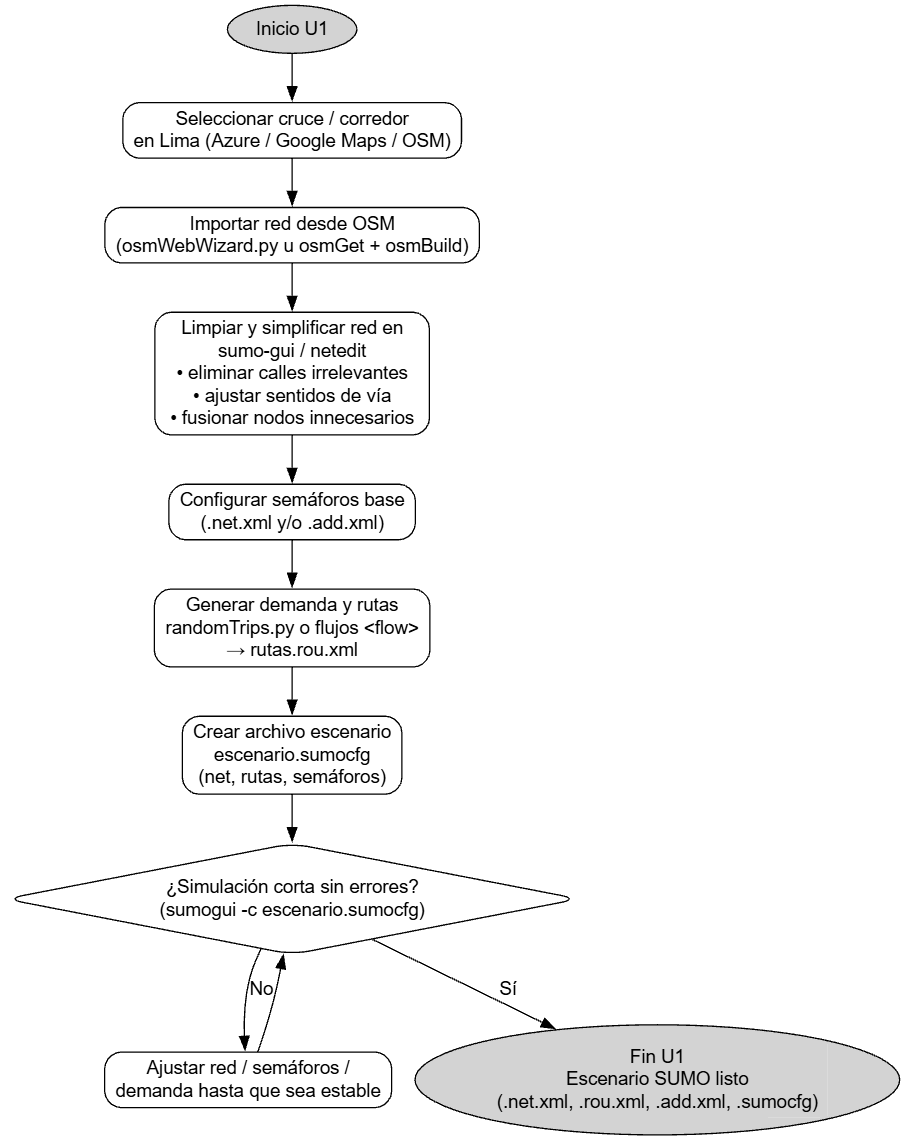
\includegraphics[width=\textwidth]{U1.png}
    \caption{Diagrama de flujo del módulo U1: preprocesamiento y generación del
    escenario SUMO.}
    \label{fig:flow-u1}
\end{figure}

\section{Resumen de las unidades}

\begin{description}
  \item[U1:] Instalar y configurar SUMO; importar la intersección
    mediante el asistente OSM o descarga manual; limpiar y validar
    la red; generar la demanda vehicular y el archivo de configuración
    \texttt{.sumocfg}.  El resultado es un escenario reproducible.
  \item[U2:] Ejecutar el escenario con TraCI y entrenar un agente de
    aprendizaje por refuerzo que ajuste las fases semafóricas.  U2
    depende exclusivamente de los archivos generados en U1 y no
    modifica la red ni las rutas.
  \item[U3:] Medir el desempeño de cada control con las mismas salidas
    de SUMO (viajes por vehículo, colas por TraCI, emisiones) y
    compararlo con el protocolo del plan de pruebas
    (Secciones~\ref{sec:u3} y~\ref{sec:plan}).
  \item[U4:] Coordinar los agentes de semáforos vecinos: estado
    continuo con la información del vecino, mensajería entre cruces,
    recompensa con penalización por \textit{spillback} y aprendizaje
    con IPPO (Sección~\ref{sec:u4}).
\end{description}

%----------------------------------------------------------------------
\section{Desarrollo del módulo U2: Aprendizaje por Refuerzo para el control de semáforos}

El segundo módulo de la metodología aborda el diseño e
implementación de un controlador inteligente que modifique las fases
de los semáforos en función del estado del tráfico. Para ello se
recurre a técnicas de \emph{Aprendizaje por Refuerzo} (\emph{Reinforcement
Learning}, RL), en las que un agente aprende a tomar decisiones
mediante la interacción con un entorno simulado. Este apartado
describe la formulación del problema, la interfaz con SUMO y los
algoritmos de RL más habituales para el control de intersecciones.

\subsection*{Formulación del problema}

En RL se define un \emph{entorno} compuesto por un conjunto de
\emph{estados}, un conjunto de \emph{acciones} y una función de
\emph{recompensa}. La formulación implementada en esta tesis para un
cruce con cuatro aproximaciones es la siguiente:

\begin{itemize}
  \item \textbf{Estado:} el número de vehículos detenidos en cada
    aproximación, leído con \verb|edge.getLastStepHaltingNumber| y
    discretizado en cuatro niveles (0; 1 a 3; 4 a 8; más de 8), más el
    índice de la fase verde activa. El estado es $s = (c_N, c_S, c_E,
    c_O, f)$ con $c_i \in \{0,1,2,3\}$. Con dos fases verdes el espacio
    tiene $4^4 \times 2 = 512$ estados y con cuatro fases, $1024$. Esta
    discretización es la que hace viable una tabla Q y, a la vez, la
    que limita al método tabular cuando crece el número de fases, como
    se muestra en el Capítulo~\ref{cap:resultados}.

  \item \textbf{Acción:} dos acciones. $a = 0$ mantiene la fase verde
    actual y $a = 1$ pasa a la siguiente fase verde del programa,
    insertando automáticamente el ámbar del programa (3~s). El agente
    no elige una fase arbitraria ni una duración: decide únicamente
    cuándo termina el verde en curso.

  \item \textbf{Recompensa:} negativa y proporcional a la congestión en
    el instante de la decisión,
    \begin{equation}
      r = -\Bigl(w_1 \sum_i c_i + w_2 \sum_i e_i\Bigr), \qquad
      w_1 = 1.0,\; w_2 = 0.01,
      \label{eq:recompensa}
    \end{equation}
    donde $c_i$ es el número de vehículos detenidos en la aproximación
    $i$ (sin discretizar) y $e_i$ es la suma de los tiempos de espera de
    los vehículos que en ese momento están en la aproximación $i$
    (\verb|edge.getWaitingTime|). Con estos pesos domina el término de
    colas; el de espera desempata entre estados con la misma cola. La
    recompensa mide el nivel de congestión, no su incremento entre
    decisiones. Es la recompensa de la fase exploratoria. En el plan de
    pruebas vigente (Sección~\ref{sec:plan2}) Q-learning y SARSA se
    entrenan con la recompensa de retraso de la
    Ecuación~\ref{eq:recompensa-u4}, la misma de DQN, IPPO y MAPPO; la
    de la Ecuación~\ref{eq:recompensa} se conserva solo en la ablación
    \texttt{ql\_colas}.

  \item \textbf{Restricciones operativas:} el verde dura al menos 10~s
    antes de que el agente pueda cambiarlo (5~s en las fases de giro
    protegido, identificadas por tener a lo más dos movimientos en
    verde) y como máximo 60~s, tras los cuales el cambio se fuerza. El
    agente decide cada 5~s.
\end{itemize}

Con estos elementos se modela el control del semáforo como un
\emph{problema de decisión de Markov} (MDP). El agente observa el
estado, aplica una acción, avanza la simulación y recibe una
recompensa; a partir de la secuencia de experiencias va aprendiendo
una política de control. En los escenarios con varios cruces se
instancia un agente por semáforo, cada uno con su propia tabla Q, su
estado local y su recompensa local; los agentes no intercambian
información (eso es lo que añade el módulo U4).

\subsection*{Interfaz con SUMO y ciclo de entrenamiento}

Para implementar el bucle de RL se emplea la interfaz TraCI,
proporcionada por SUMO, que permite controlar la simulación desde
Python. El ciclo implementado consta de los siguientes pasos:

\begin{enumerate}
  \item \textbf{Inicio del episodio:} se lanza SUMO con
    \verb|traci.start| sobre el escenario de U1, con una semilla
    explícita (\verb|--seed|) y la salida por vehículo \texttt{tripinfo}
    activada. Se lee el programa del semáforo para identificar sus
    fases verdes y el ámbar que sigue a cada una, y se fija la primera
    fase verde con duración indefinida: a partir de ahí el agente
    decide cuándo cambia.
  \item \textbf{Decisión cada 5~s:} se lee el estado (colas
    discretizadas y fase activa) y se elige la acción con una política
    $\varepsilon$-greedy: con probabilidad $\varepsilon$ una acción al
    azar y, si no, la de mayor valor Q, desempatando al azar cuando
    ambas valen lo mismo. Si la acción es cambiar y el verde lleva al
    menos el mínimo, se activa el ámbar con \verb|trafficlight.setPhase|
    y \verb|setPhaseDuration|, se avanza la simulación esos segundos y
    se entra al siguiente verde. Luego se avanzan 5~s con
    \verb|simulationStep|.
  \item \textbf{Recompensa y actualización:} con el estado resultante
    se calcula la recompensa de la ecuación~\ref{eq:recompensa} y, en
    entrenamiento, se actualiza $Q(s,a)$ con la regla de Q-learning
    ($\alpha = 0.1$, $\gamma = 0.9$).
  \item \textbf{Fin del episodio:} cuando no quedan vehículos por
    insertar ni circulando (\verb|simulation.getMinExpectedNumber|
    igual a cero) o al llegar a 6000 pasos, se cierra SUMO con
    \verb|traci.close|, se leen del \texttt{tripinfo} las métricas del
    episodio (Sección~\ref{sec:u3}) y se guarda la tabla Q en disco.
\end{enumerate}

\noindent\textbf{Qué es un episodio y qué cambia entre episodios.}
Un episodio es una simulación completa de una hora de tráfico (0 a
3600~s de demanda, más el tiempo necesario para que salgan los últimos
vehículos) sobre la misma red y la misma demanda. Dentro de la hora el
agente toma del orden de 600 a 800 decisiones por semáforo y actualiza
su tabla Q en cada una. Entre un episodio y el siguiente cambian
exactamente tres cosas:

\begin{itemize}
  \item la probabilidad de exploración $\varepsilon$, que arranca en 1.0
    y se multiplica por 0.9 al terminar cada episodio hasta un piso de
    0.05 (lo alcanza en el episodio 30; con los decaimientos más lentos
    usados en los escenarios grandes, 0.96 y 0.95, lo alcanza en los
    episodios 75 y 60);
  \item la semilla de SUMO, que vale la semilla base más el número de
    episodio;
  \item la tabla Q, que el agente hereda del episodio anterior.
\end{itemize}

La demanda es idéntica en todos los episodios: los flujos se definen
con \verb|vehsPerHour|, que inserta los vehículos equiespaciados, de
modo que la semilla solo altera el comportamiento de los conductores
(su factor de velocidad individual y la imperfección $\sigma$ del modelo
de seguimiento), no cuántos vehículos llegan ni cuándo. No se ajustan
$\alpha$, $\gamma$ ni los pesos de la recompensa entre episodios.

El número de episodios se fija por el schedule de $\varepsilon$: los
necesarios para que llegue al piso, más al menos diez de consolidación
en los que el agente casi solo explota lo aprendido. Con decaimiento
0.9 son 40 episodios; con 0.96, 120; con 0.95, 100. Estos valores son
los de la fase exploratoria: en el plan de pruebas vigente todos los
aprendices se entrenan 200 episodios, con el decaimiento y el piso de
$\varepsilon$ de la Sección~\ref{sec:plan2}. Para comprobar que
ese criterio basta se registran por episodio el número de estados
distintos visitados y el mayor cambio de un valor Q, y cada cinco
episodios se evalúa la política congelada ($\varepsilon = 0$) sobre una
copia de la tabla Q, con una semilla fija ajena al entrenamiento y sin
alterar el generador aleatorio del entrenamiento. Las métricas de los
episodios de entrenamiento describen el proceso de aprendizaje, con
exploración y con la tabla Q cambiando dentro de la hora; el resultado
del agente se mide aparte, con la política congelada y varias semillas,
según el plan de pruebas de la Sección~\ref{sec:plan}.

El núcleo del ciclo, simplificado a partir de la función
\texttt{correr\_episodio} de \texttt{rl\_semaforo.py} (Anexo~B), es el
siguiente:

{\footnotesize\begin{verbatim}
traci.start(["sumo", "-c", CFG, "--seed", str(seed),
             "--tripinfo-output", tripinfo])
verdes, ambar, dur_ambar, verde_min = fases_verdes()  # fases del programa
verde, t_verde, pasos = 0, 0, 0
poner_fase(verdes[verde], 100000)     # el agente decide cuando cambiar
s = estado(verde)
while traci.simulation.getMinExpectedNumber() > 0 and pasos < 6000:
    if modo == "train" and random.random() < eps:
        a = random.randint(0, 1)      # exploracion
    else:
        a = mejor_accion(Q, s)        # explotacion (desempate al azar)
    cambiar = (a == 1 and t_verde >= verde_min[verdes[verde]]) \
              or t_verde >= VERDE_MAX
    if cambiar:
        f = verdes[verde]
        poner_fase(ambar[f], dur_ambar[f])
        avanzar(dur_ambar[f])         # ambar de 3 s
        verde = (verde + 1) % len(verdes)
        poner_fase(verdes[verde], 100000)
        t_verde = 0
    avanzar(PASO_CONTROL)             # 5 s de simulacion
    t_verde += PASO_CONTROL
    r = recompensa()                  # -(w1 * colas + w2 * esperas)
    s2 = estado(verde)
    if modo == "train":
        q = q_vals(Q, s)
        q[a] += ALPHA * (r + GAMMA * max(q_vals(Q, s2)) - q[a])
    s = s2
traci.close()
\end{verbatim}
}

El mismo bucle sirve para los controles de referencia (tiempo fijo y
actuado): en esos modos el semáforo corre su propio programa y el
código solo mide, con la misma recompensa y las mismas métricas. El
script completo, con los modos \texttt{baseline}, \texttt{actuado},
\texttt{train} y \texttt{demo}, se incluye en el Anexo~B.

En los escenarios con varios semáforos el bucle es el mismo, con un
agente y una tabla Q por intersección. Cada agente lleva su propio
reloj de decisión, contado desde el inicio de su verde, de modo que el
verde mínimo se respete por igual en todos ellos, y no decide mientras
su semáforo está en ámbar. Los agentes no intercambian información: la
única forma en que un cruce percibe a su vecino es a través de las
colas que le llegan. La primera decisión de cada verde, a los 5~s, está
siempre forzada a mantener por el verde mínimo; el módulo U4
(Sección~\ref{sec:u4}) conserva este reloj y añade la comunicación
entre vecinos.

\subsection*{Algoritmos recomendados}

Diversas técnicas de RL han sido aplicadas al control de
semáforos. Los algoritmos tabulares, como \emph{Q-learning} o
\emph{SARSA}, son adecuados para intersecciones sencillas con un
número limitado de estados, y son los que permiten inspeccionar
directamente la política aprendida. Para espacios de estado mayores se
emplean métodos de \emph{Deep Reinforcement Learning} como \emph{Deep
Q-Network} (DQN) y \emph{Proximal Policy Optimization} (PPO), que
sustituyen la tabla por una red neuronal capaz de generalizar entre
estados parecidos. Ambos tienen implementación de referencia en
\texttt{stable-baselines3}, sobre PyTorch, y su acoplamiento a SUMO
reutiliza el mismo bucle de TraCI descrito arriba.

En esta fase se implementaron los cuatro, sin
\texttt{stable-baselines3}: Q-learning y SARSA tabulares (este módulo,
\texttt{rl\_corredor.py}), PPO en su versión multiagente independiente
(IPPO, módulo U4, Sección~\ref{sec:u4}) y, para el plan de pruebas, un
Double DQN y un MAPPO en PyTorch puro (Sección~\ref{sec:plan2}).
La motivación para pasar de la tabla a la red está en los resultados
del Capítulo~\ref{cap:resultados}: la representación tabular alcanza su
techo en cuanto crece el número de fases del semáforo, que es
exactamente el caso en que la aproximación por redes neuronales resulta
pertinente.

\subsection*{Actualización de los valores Q y ejemplo de pseudocódigo}

En el caso de algoritmos tabulares, como Q-learning, la política del agente se
representa mediante una \emph{tabla Q} en la que cada entrada $Q(s,a)$
almacena la expectativa de recompensa acumulada si se aplica la acción $a$ en
el estado $s$ y se sigue la mejor política a partir de entonces.
El proceso de aprendizaje consiste en actualizar iterativamente estos valores
con información obtenida de las simulaciones.  La regla de actualización de
Q-learning se basa en el aprendizaje por diferencias temporales y se expresa
de la siguiente manera:

\[
  Q(s,a) \leftarrow Q(s,a) + \alpha \bigl[r + \gamma\,\max_{a'} Q(s',a') - Q(s,a)\bigr],
\]
donde $\alpha$ es la tasa de aprendizaje, $\gamma$ el factor de descuento,
$r$ la recompensa inmediata obtenida al ejecutar la acción $a$ en el estado $s$,
$s'$ el estado siguiente y $a'$ las posibles acciones en $s'$.  Esta
ecuación desplaza el valor Q actual en dirección del retorno observado
($r + \gamma \max_{a'} Q(s',a')$).

Para algoritmos \emph{on--policy}, como SARSA, la actualización se realiza con la
siguiente fórmula:

\[
  Q(s,a) \leftarrow Q(s,a) + \alpha\bigl[r + \gamma\,Q(s',a') - Q(s,a)\bigr],
\]

donde $a'$ es la acción efectivamente seleccionada en el estado siguiente $s'$
y $\alpha,\gamma$ tienen el mismo significado que en Q-learning.  Al emplear
el valor $Q(s',a')$ asociado a la política vigente en vez del máximo de todas
las acciones, SARSA mantiene la coherencia entre exploración y actualización
y suele conducir a comportamientos más conservadores.

\subsection*{Diagrama de flujo del módulo U2}

La Figura~\ref{fig:flow-u2} sintetiza el ciclo de entrenamiento del módulo U2.
A partir del escenario generado en U1, el agente de RL interactúa con SUMO a
través de TraCI, observa el estado del tráfico, selecciona acciones sobre el
semáforo, actualiza sus valores $Q(s,a)$ (o los parámetros de la red neuronal)
y registra métricas de desempeño por episodio.
\begin{figure}[H]
    \centering
    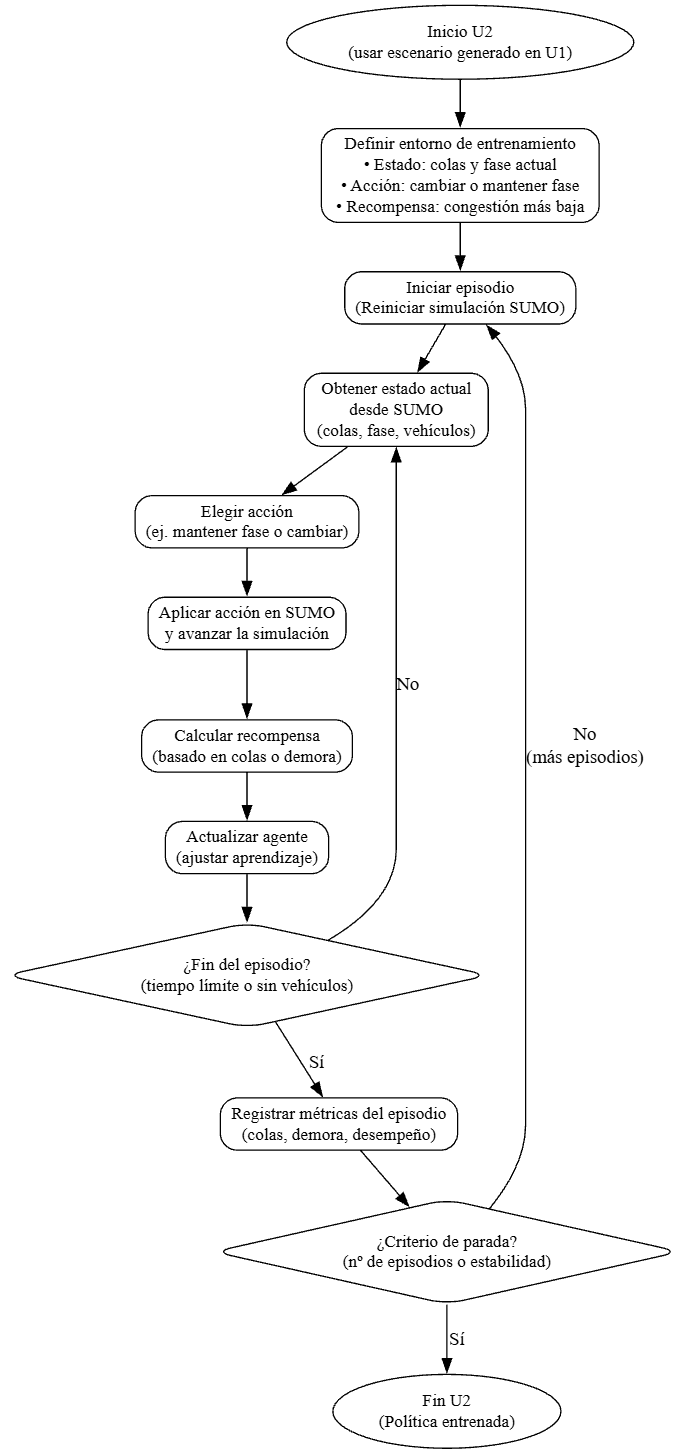
\includegraphics[width=0.62\textwidth]{U2.png}
    \caption{Diagrama de flujo del módulo U2: entrenamiento del agente de
    Aprendizaje por Refuerzo para el control semafórico.}
    \label{fig:flow-u2}
\end{figure}

%----------------------------------------------------------------------
\section{Módulo U3: medición del desempeño}
\label{sec:u3}

Todas las métricas se calculan con las mismas salidas de SUMO para los
tres controles comparados (tiempo fijo, actuado y agente RL), de modo
que la comparación no dependa de cómo decide cada uno.

\begin{itemize}
  \item \textbf{Por vehículo}, del archivo \texttt{tripinfo} que SUMO
    escribe al terminar cada viaje: el retraso (\texttt{timeLoss}), la
    espera detenida (\texttt{waitingTime}), el número de paradas
    (\texttt{waitingCount}, veces que la velocidad bajó de 0.1~m/s) y
    el instante de llegada. El \textit{throughput} se define como el
    número de vehículos que completan su viaje antes de los 3600~s. Con
    el dispositivo de emisiones activado
    (\verb|--device.emissions.probability 1|) cada viaje incluye además
    sus emisiones acumuladas; se reportan CO$_2$ en gramos y NO$_x$ en
    miligramos por vehículo, con la clase de emisión por defecto de SUMO
    (HBEFA3, turismo a gasolina Euro~4) \citep{SUMO_Emissions}. Activar
    el dispositivo no altera la dinámica ni la secuencia aleatoria de la
    simulación: las métricas con y sin él coinciden.
  \item \textbf{Por segundo}, vía TraCI: el número de vehículos
    detenidos, sumado sobre todas las aproximaciones semaforizadas del
    escenario. De esa serie salen la cola promedio, que es su media por
    segundo de simulación, y la cola máxima, que es su mayor valor
    instantáneo; se guarda además un muestreo por minuto para observar
    la respuesta de cada control al cambio de demanda.
  \item \textbf{Por decisión}: la recompensa de la
    Ecuación~\ref{eq:recompensa} se evalúa cada 5~s de reloj fijo, con
    el mismo muestreo bajo los tres controles, para comparar lo que el
    agente optimiza con lo que consiguen el fijo y el actuado. Se
    reporta como promedio por decisión y no como suma acumulada, para
    que el valor no dependa de la duración del episodio. Se cuentan
    además los cambios de fase (entradas a una fase verde) de cada
    control, sobre el episodio completo.
  \item \textbf{Retornos por segundo}, desde el plan de pruebas
    vigente: tres recompensas (de retraso, de colas y de
    \textit{spillback}) acumuladas cada segundo sobre todos los
    semáforos, con cualquier control. Se definen en la
    Sección~\ref{sec:plan2}.
\end{itemize}

\subsection*{Métricas de corredor y \textit{spillback}}

En los escenarios de varios cruces se miden además, con las mismas
salidas y para todos los controles, las magnitudes que la coordinación
debería mover. Del \texttt{tripinfo}, sobre los vehículos que recorren
la avenida de extremo a extremo (850 en corredor, unos 900 en red): el
tiempo de viaje y el retraso medios, el retraso medio en el sentido de
la punta (el que favorece la onda verde del programa fijo), las paradas
medias y la fracción de vehículos que se detiene a lo sumo una vez,
que es el indicador más directo de progresión. Por TraCI, en cada
carril de los enlaces que unen dos cruces: el máximo de vehículos
detenidos y el máximo de vehículos presentes durante la corrida, y el
\textit{spillback}, definido como un segundo en el que algún carril de
algún enlace tiene detenidos al menos el 90\,\% de sus plazas (34 de
38: la cola queda a menos de 30~m del cruce aguas arriba y el siguiente
vehículo que se detenga bloquea la intersección). Se reportan la
fracción de segundos de la hora con \textit{spillback}, los segundos
totales y el número de episodios de \textit{spillback} (flancos de
subida). Se cuenta también el número de vehículos que no terminaron su
viaje al cerrar la simulación, que es cero con la demanda nominal. Al
pedir la serie se guarda además la fase de cada semáforo en cada
segundo, para observar el desfase que emerge entre cruces.

Dos precisiones importan para leer los resultados. El retraso de SUMO
incluye tiempo perdido que no depende del semáforo (arranque desde
velocidad cero, giros a menor velocidad, vacilaciones del conductor),
así que un cambio porcentual sobre \texttt{timeLoss} subestima el
efecto sobre el retraso atribuible al control. Y la espera detenida es
la señal que optimiza la recompensa, pero no es el retraso: un control
que fragmenta las colas en paradas más cortas puede bajar la espera y
subir las paradas sin mover el retraso. Por eso el retraso es la
métrica primaria y la espera, las colas, las paradas, el
\textit{throughput} y las emisiones son secundarias.

%----------------------------------------------------------------------
\section{Desarrollo del módulo U4: coordinación distribuida entre semáforos}
\label{sec:u4}

Los resultados del módulo U2 en los escenarios de varios cruces
(Capítulo~\ref{cap:resultados}) motivan este módulo: tres agentes
tabulares independientes pierden un $15$\,\% de retraso frente a la onda
verde tuneada de red, dos agentes en el corredor pierden un $60$\,\%
frente al fijo con reparto de verde tuneado (un $6$\,\% frente al fijo
simétrico de la primera ronda) y su política resultó sensible a un
cambio de 2~s en el verde mínimo. El
módulo U4 cambia cuatro cosas a la vez, de forma incremental y
comparable: el estado pasa de bins a un vector continuo que incluye lo
que el propio detector ve en movimiento; cada semáforo recibe mensajes
de sus vecinos sobre la avenida; la recompensa puede penalizar la cola
que el agente empuja sobre el enlace que comparte con el vecino
(\textit{spillback}); y el aprendizaje pasa de la tabla Q a
\emph{Independent PPO} (IPPO) con una sola red compartida por todos los
semáforos. Todo se implementa en \texttt{rl\_ippo.py} (Anexo~B) sobre
PyTorch en CPU, sin Gym ni \texttt{stable-baselines3}, reutilizando el
bucle de TraCI, el reloj de decisión y las métricas de U2 y U3.

\subsection*{Vecinos y canal de mensajes}

Dos semáforos son vecinos cuando comparten un tramo de la avenida: en
corredor C1 y C2; en red C1--C2 y C2--C3 (la rotonda no tiene semáforo
y no participa). En la malla de nueve cruces del plan de pruebas (P5)
cada semáforo tiene de dos a cuatro vecinos, uno por lado
(Sección~\ref{sec:plan2}). Cada 5~s de reloj global, cada semáforo publica a cada
vecino un mensaje con cinco datos que un controlador real podría
transmitir: la fase en curso (avenida, transversal o ámbar), el tiempo
que lleva en ella, los vehículos presentes en la aproximación que
descarga hacia el vecino, la cola detenida en esa aproximación y la
cola detenida en el enlace que une al emisor con el receptor, que es
el enlace por el que llegan al receptor esos vehículos. El receptor
conserva el último mensaje recibido y su edad. El canal admite una
latencia fija y una probabilidad de pérdida por mensaje, ambas nulas
durante el entrenamiento y usadas solo en la prueba de robustez del
plan de pruebas; la pérdida usa un generador aleatorio propio para no
alterar la secuencia de la simulación.

\subsection*{Observación, acciones y máscara}

La observación de cada agente es un vector de 31 componentes
normalizadas entre 0 y 1 (Tabla~\ref{tab:obs-u4}): un bloque local de
15 y dos ranuras fijas de 8, una para el vecino del oeste y otra para
el del este. Las colas se dividen por la capacidad de la aproximación
(plazas de 7.5~m por carril) y la cola del enlace por sus plazas
(38 en los enlaces de 300~m). La variante \emph{local} deja las dos
ranuras a cero: contiene todo lo que un detector propio puede medir, de
modo que la diferencia entre \emph{vecinos} y \emph{local} se atribuye
solo a la mensajería. La misma red y la misma disposición sirven para
los tres escenarios; el identificador del semáforo ocupa tres
posiciones fijas. En la malla del plan de pruebas (P5) la disposición
se extiende sin cambiar el bloque local: nueve posiciones de
identificador y cuatro ranuras de 8 (oeste, este, norte y sur), 53
componentes en total; ``verde hacia mí'' es el verde este--oeste para
un vecino al oeste o al este y el norte--sur para uno al norte o al
sur. Con dos lados la disposición sigue siendo la de la tabla, y las
políticas anteriores cargan sin cambios.

\begin{table}[H]
\centering
\scriptsize
\setlength{\tabcolsep}{3pt}
\begin{spacing}{1}
\begin{tabular}{llp{9.2cm}}
\toprule
Bloque & Componentes & Contenido \\
\midrule
Local & 1--4 & cola detenida en cada aproximación (O, E, N, S) sobre su capacidad \\
 & 5--8 & vehículos en movimiento en cada aproximación sobre su capacidad \\
 & 9--10 & fase verde activa (uno de dos) \\
 & 11 & tiempo en el verde actual sobre 60~s \\
 & 12 & 1 si ya se cumplió el verde mínimo \\
 & 13--15 & identificador del semáforo (uno de tres) \\
\midrule
Vecino oeste & 16 & 1 si existe el vecino \\
(17--22 a cero si & 17 & 1 si el vecino está en la fase de la avenida (descarga hacia mí) \\
no hay mensaje) & 18 & 1 si el vecino está en ámbar \\
 & 19 & tiempo del vecino en su fase sobre 60~s \\
 & 20 & vehículos en la aproximación del vecino que descarga hacia mí, sobre su capacidad; cero si el vecino no está en la fase de la avenida \\
 & 21 & cola detenida en esa aproximación sobre su capacidad \\
 & 22 & cola detenida en el enlace que llega desde el vecino (del vecino hacia mí), máximo por carril, sobre sus plazas \\
 & 23 & edad del último mensaje sobre 30~s (1 si nunca llegó) \\
\midrule
Vecino este & 24--31 & igual que 16--23 \\
\bottomrule
\end{tabular}
\end{spacing}
\caption{Observación de cada agente del módulo U4.}
\label{tab:obs-u4}
\end{table}

La componente 22 (y la 30) se llama \texttt{cola\_mi\_salida} en el
código porque se diseñó para medir la cola del enlace que el agente
alimenta hacia el vecino, la que anticipa el \textit{spillback} que él
mismo provoca. La implementación, heredada de la fase del 06.09.2026,
mide el enlace en el sentido contrario: el que llega desde el vecino,
que es una de las aproximaciones del propio agente y que el bloque
local ya ve en parte (componentes 1 a 4). La normalización usa las
plazas del enlace de salida, pero los dos sentidos de cada enlace
tienen la misma longitud en todos los escenarios (38 plazas por carril
en corredor y red, 37 en malla3), así que el valor numérico es
correcto para lo que mide. Todas las políticas de IPPO, DQN y MAPPO de
este documento se entrenaron con esa componente. La cola del enlace de
salida solo llega al agente a través del término de
\textit{spillback} de la variante \emph{spill}.
% fuente: rl_ippo.py, funciones mensaje (cola_salida = enlace emisor->receptor) y observar (componente base+6)

Las acciones son las de U2: mantener el verde o pasar a la siguiente
fase con ámbar automático. El verde mínimo y máximo se imponen con una
máscara sobre las acciones: antes del mínimo solo es válida mantener,
a los 60~s solo cambiar, y entre ambos las dos. Las decisiones forzadas
por la máscara no aportan gradiente a la política (su probabilidad es
1) pero sí al crítico. Se reportan por episodio las decisiones totales,
comparables con U2, y las decisiones libres.

\subsection*{Recompensa y variantes}

La recompensa de U4 conserva la estructura y los pesos de la
Ecuación~\ref{eq:recompensa} ($w_1 = 1$, $w_2 = 0.01$) con dos cambios
que salieron de la prueba de humo del plan de pruebas (más abajo). El
término de cola detenida se sustituye por los vehículos-equivalentes
retrasados de cada aproximación, $n_a\,(1 - \bar v_a / v_{\max,a})$,
donde $n_a$ es el número de vehículos presentes y $\bar v_a$ su
velocidad media: un vehículo detenido cuenta 1 y uno que avanza a
media velocidad cuenta 0.5. Es la versión por segundo del
\texttt{timeLoss} de SUMO, la métrica primaria, y se lee de la misma
suscripción por aproximación. Y el agente recibe, por cada transición,
la suma por segundo de esa cantidad sobre su intervalo de decisión
dividida entre 5~s (retraso-segundos), en lugar del nivel en el
siguiente instante de decisión: en un intervalo de mantener coincide
con el nivel medio y en uno de cambiar, de 8~s, pesa $8/5$. La variante
\emph{spill} le resta además un término por la cola que el agente
empuja sobre cada enlace que alimenta hacia un vecino, acumulado de la
misma forma:
\begin{equation}
  \begin{aligned}
  r_i = -\frac{1}{5}\sum_{t \in \text{intervalo}} \Bigl[\;
        & w_1 \sum_a n_a(t)\Bigl(1 - \frac{\bar v_a(t)}{v_{\max,a}}\Bigr)
        + w_2 \sum_a \text{espera}_a(t) \\
        & + w_3 \sum_{e \in \text{salidas}_i} \max\bigl(0,\; q_e(t) - P_e/2\bigr) \Bigr],
  \end{aligned}
  \label{eq:recompensa-u4}
\end{equation}
donde $q_e$ es el máximo por carril de vehículos detenidos en el enlace
$e$, $P_e$ sus plazas por carril (38; 37 en malla3) y $w_3 = 2$ (cero en \emph{local} y
\emph{vecinos}): el agente aguas arriba ve la cola que bloquea al
vecino como si fuera propia, con peso doble, desde que ocupa la mitad
del enlace. La variante \emph{cambio}, opcional, resta $w_4 = 2$ por
cada cambio de fase ejecutado, elegido o forzado, y se corre aparte
porque cambia el objetivo. Los pesos están fijados de antemano, sin
barrido. Lo que ve el algoritmo es la recompensa multiplicada por
0.02; en el registro por episodio se conserva la recompensa de U2
(colas detenidas) a reloj fijo de 5~s, comparable con los cuatro casos
ya evaluados, y aparte la recompensa completa que vio el agente.

\subsection*{Algoritmo: IPPO con pesos compartidos}

Cada semáforo es un agente independiente que decide con su propia
observación, y todos comparten los mismos parámetros: un actor
(31--64--64--2) y un crítico (31--64--64--1), perceptrones con
activación tangente hiperbólica e inicialización ortogonal, 12\,611
parámetros en total. El crítico usa la misma observación que el actor
(descentralizado), lo que hace del método un IPPO y no un MAPPO. En
cada paso de simulación los agentes en instante de decisión se evalúan
en un solo lote; en entrenamiento la acción se muestrea de la política
enmascarada y en evaluación se toma la de mayor probabilidad, el
equivalente exacto de $\varepsilon = 0$ en U2. Al terminar el episodio
se calculan por agente las ventajas por GAE y, si la red se vació, el
valor final es cero; si el episodio se cortó a 6000 pasos se usa el
valor estimado del estado final. Las trayectorias de todos los agentes
se concatenan en un lote (unas 1250 transiciones en corredor y 1900 en
red), se normalizan las ventajas y se hace una actualización PPO por
episodio con los hiperparámetros de la Tabla~\ref{tab:hiper-ippo}. Los
intervalos de 5~s (mantener) y 8~s (cambiar) se tratan como un paso
con el mismo descuento, igual que en U2.

\subsection*{Lo que enseñó la prueba de humo}

Antes de entrenar en los escenarios de varios cruces, el plan de
pruebas exige que la variante \emph{local} baje del fijo en el cruce
de dos fases (23.2~s) con 60 episodios. La primera versión, escrita con
la recompensa de U2 y los hiperparámetros habituales de PPO (tasa
$3\times10^{-4}$, minilote 256, 8 épocas, recorte de gradiente global),
falló tres veces, y cada fallo cambió una decisión de diseño que aquí
se deja registrada:

\begin{enumerate}
  \item \textbf{Recorte de gradiente por red.} La política colapsó a
    cambiar de fase en cuanto lo permitía el verde mínimo (131~s de
    retraso, cinco veces el fijo) y la red terminó ignorando la
    observación. El error inicial del crítico (retornos de $-20$ a
    $-30$ frente a un valor inicial de cero) hacía su gradiente unas
    130 veces mayor que el del actor, y el recorte conjunto reducía el
    paso del actor 50 veces. Se recortan las dos redes por separado.
  \item \textbf{Retraso en lugar de cola detenida.} Con el recorte
    corregido la política siguió derivando hacia cambiar. La causa está
    en la señal: SUMO cuenta como detenido a un vehículo con velocidad
    menor que 0.1~m/s, así que cuando el verde cambia muy seguido las
    colas reptan en vez de pararse y desaparecen del conteo sin haber
    salido; bajo esa política el retraso por vehículo era 9.6 veces la
    cola detenida media, contra 4.4 bajo el fijo. El agente tabular no
    cayó en ese óptimo local porque explora y valora estado por estado;
    un optimizador de gradiente sigue la pendiente local desde una
    política aleatoria, que en este cruce está ya saturada. Con los
    vehículos-equivalentes retrasados de la Ecuación~\ref{eq:recompensa-u4}
    la deriva desapareció.
  \item \textbf{Presupuesto de optimización por episodio.} Con la
    recompensa corregida la política dejó de empeorar, pero en 60
    episodios no salió de un programa de verdes largos (36.4~s en la
    evaluación intermedia, sin cambio entre los episodios 10 y 60): el
    cambio de la política por actualización, medido como divergencia
    entre la política vieja y la nueva, tenía una mediana de 0.0003 y
    quedaba por debajo de 0.001 en el 82\,\% de los episodios, con 24
    pasos de gradiente por episodio (3 minilotes por 8 épocas). Con
    tasa $10^{-3}$, minilote 64 y 10 épocas (unos 100 pasos por
    episodio) la evaluación intermedia iguala
    al actuado (15.4~s frente a 15.5) en 15 episodios y termina en
    14.8~s; bajar $\gamma$ y $\lambda$ a 0.9 sin tocar el presupuesto
    llega a 19.9~s en 60 episodios y no aporta nada sobre lo anterior,
    así que se conservan los valores de 0.95.
\end{enumerate}

Los tres ajustes se hicieron en el cruce de un semáforo, que no forma
parte de los casos de U4: las corridas que fallaron usaron la semilla
base 42 y las tres de ajuste de hiperparámetros, las bases 43 a 45.
Quedaron congelados antes de entrenar en corredor y red. Con ellos, la corrida formal de la prueba de humo
(semilla base 42, 60 episodios) supera la compuerta con margen: la
política congelada evaluada con las diez semillas del protocolo da
$15.05 \pm 0.21$~s de retraso, un $-35$\,\% frente al fijo, al nivel
del actuado ($15.46$~s) y muy por debajo del Q-learning ($21.72$~s); el
detalle está en el Capítulo~\ref{cap:resultados}. Los registros de las
corridas fallidas están en la carpeta \texttt{humo/} del proyecto.

\begin{table}[H]
\centering
\scriptsize
\setlength{\tabcolsep}{3pt}
\begin{spacing}{1}
\begin{tabular}{lll}
\toprule
Hiperparámetro & Valor & Comentario \\
\midrule
Descuento $\gamma$ & 0.95 & horizonte de unas 20 decisiones (100~s), cubre el viaje entre cruces \\
GAE $\lambda$ & 0.95 & \\
Recorte de PPO & 0.2 & \\
Épocas por actualización & 10 & fijado en la prueba de humo (8 en la propuesta inicial) \\
Minilote & 64 & fijado en la prueba de humo (256 en la propuesta inicial) \\
Tasa de aprendizaje & $10^{-3}$ & Adam, decaimiento lineal hasta 0; $3\times10^{-4}$ en la propuesta inicial \\
Coeficiente de entropía & 0.01 & \\
Coeficiente del valor & 0.5 & pérdida cuadrática sin recorte \\
Recorte de gradiente & 0.5 & norma por red (actor y crítico por separado) \\
Escala de la recompensa & 0.02 & constante, sin normalización adaptativa \\
Episodios & 200 & semillas de SUMO base$+1$ a base$+200$ \\
Evaluación intermedia & cada 10 & política congelada con la semilla 999 \\
Semillas base & 42, 2042, 4042 & tres entrenamientos por variante y escenario \\
\bottomrule
\end{tabular}
\end{spacing}
\caption{Hiperparámetros de IPPO.}
\label{tab:hiper-ippo}
\end{table}

Se entrenan tres políticas por variante y escenario, con semillas base
distintas cuyos rangos no se solapan entre sí ni con las semillas de
evaluación. La política que representa a cada variante en las tablas
principales es la de la semilla base cuya última evaluación intermedia
es la mediana de las tres; las otras dos se reportan en el anexo y el
rango entre las tres mide la fragilidad del entrenamiento, que fue el
hallazgo del corredor en U2. El entrenamiento es determinista: siembra
los generadores de Python, NumPy y PyTorch con la semilla base, usa un
solo hilo y algoritmos deterministas, y repetir una corrida reproduce
el registro por episodio dígito a dígito. Cada política se guarda con
un archivo de metadatos (escenario, variante, semilla base,
hiperparámetros, capacidades, tabla de vecinos y versiones de software)
que basta para reproducir su evaluación.

\subsection*{Escenario de estrés corredor\_alta}

Con la demanda nominal de corredor y red ninguna cola detenida llega a
ocupar el enlace entre cruces (en promedio 16 y como máximo 20 de las
38 plazas del enlace en corredor bajo el fijo), así que el término de \textit{spillback} no se activaría y
el \textit{throughput} no discrimina. Se define por eso un escenario
de estrés, corredor\_alta, con la misma red y el mismo patrón de
corredor y todos los flujos multiplicados por un factor $f$. El factor
se eligió antes de entrenar nada, con el control actuado sobre tres
semillas ajenas a las de evaluación (2001 a 2003) y el criterio
prefijado de tomar el menor $f$ de $\{1.3, 1.5, 2.0\}$ con el que la
cola detenida en algún carril de los enlaces alcanza el umbral de
\textit{spillback} (34 de 38 plazas) en al menos dos de las tres
semillas: con 1.3 no lo alcanza en ninguna (máximos de 26, 28 y 31), con
1.5 en una (30, 32 y 35) y con 2.0 en las tres (38 en todas, con
\textit{spillback} durante 53 a 104~s de la hora). Queda $f = 2$: 3620
vehículos en la hora y 1200~veh/h en el sentido punta de la avenida,
por encima de la capacidad de un carril con la mitad del ciclo en
verde. Bajo esa demanda el programa fijo de corredor deja entre 80 y 94
vehículos sin terminar a los 6000 pasos y el actuado los termina todos,
por lo que en este escenario se reportan también el número de vehículos
no terminados, el \textit{throughput} y las diferencias absolutas de
retraso. El programa fijo se vuelve a tunear para esta demanda con un
barrido asimétrico (verde de la avenida de 25 a 40~s, verde transversal
de 10 a 25~s y desfase de 0 a 30~s, 80 configuraciones) sobre las
mismas semillas 2001 a 2003: el mejor es 25~s para la avenida, 15~s
para las transversales y desfase de 25~s, con 152~s de retraso sobre
esas semillas frente a 171~s del programa nominal de corredor; el
actuado se genera de él como en los demás casos. Los programas fijos de los cuatro
escenarios nominales se tunearon con las semillas 1001 a 1003, un
subconjunto de las de evaluación; a partir de este escenario todo tuneo
usa 2001 a 2003.

%----------------------------------------------------------------------
\section{Plan de pruebas}
\label{sec:plan}
\label{sec:plan2}

El plan de pruebas vigente, aprobado por el asesor el 23.09.2026,
aplica un mismo método en todas las configuraciones y mide las mismas
salidas en todas ellas. Cada caso fija un escenario (red y demanda);
en cada caso se entrenan y evalúan los mismos modelos con el mismo
protocolo, y un veredicto prefijado dice si el modelo funciona en ese
caso. La fase anterior, exploratoria, se resume al final de la
sección.

\subsection*{Objetivo de cada prueba}

La pregunta es la misma en todas las celdas de la matriz caso por
modelo: \emph{¿el modelo reduce el retraso por vehículo frente al
tiempo fijo tuneado en ese caso, y no queda por detrás del actuado?}
Cada caso agrega una dificultad a la anterior. P1 y P2 comparan un
corredor de dos semáforos con demanda nominal y con demanda doble, y
responden si el modelo sigue funcionando cuando la demanda supera la
capacidad de un carril. P3 y P4 repiten la comparación en la red de
tres semáforos, dos carriles por sentido y una rotonda sin semáforo,
con la demanda nominal y con una un 20\,\% mayor (el límite que impone
la rotonda), y responden si funciona con más carriles y con un
elemento que no controla. P5 pasa a una malla de nueve semáforos en la
que los cruces tienen vecinos en los dos ejes, hasta cuatro, y
responde si el método escala a una red.

\subsection*{Casos}

La Tabla~\ref{tab:plan2-casos} resume los casos. P1 a P5 se ejecutan
en esta fase. P6 (la misma malla con demanda alta) y P7 (una red de
cuatro por cuatro cruces, con tres carriles por sentido y fase de giro
protegido) quedan definidos como trabajo siguiente: repiten el mismo
protocolo sobre escenarios de mayor tamaño y no cambian el método.
La avenida es siempre el eje este--oeste y la transversal, el
norte--sur; en la malla los dos ejes tienen dos carriles y la
convención se mantiene.

\begin{table}[H]
\setstretch{1}
\centering
\footnotesize
\setlength{\tabcolsep}{4pt}
\begin{tabular}{llcclc}
\toprule
Caso & Escenario & Semáforos & \makecell{Carriles por\\sentido (avenida)} & Demanda & \makecell{Vehículos\\en la hora} \\
\midrule
P1 & corredor       & 2              & 1 & nominal                & 1810 \\
P2 & corredor\_alta & 2              & 1 & 2.0 $\times$ nominal   & 3620 \\
P3 & red            & 3 + rotonda    & 2 & nominal                & 2150 \\
P4 & red\_alta      & 3 + rotonda    & 2 & 1.2 $\times$ nominal   & 2580 \\
P5 & malla3         & 9 (3$\times$3) & 2 & nominal                & 4350 \\
\midrule
P6 & malla 3$\times$3 & 9            & 2 & alta                   & por definir \\
P7 & red 4$\times$4 & 16             & \makecell{3, con giro\\protegido} & por definir & por definir \\
\bottomrule
\end{tabular}
\caption[Casos del plan de pruebas]{Casos del plan de pruebas. P1 a P5 se ejecutan en esta
fase; P6 y P7 quedan como trabajo siguiente. Carriles por sentido en la avenida. La demanda
nominal es la de cada escenario en la Tabla~\ref{tab:escenarios} y, en malla3, la descrita en
esta sección; el factor de P4 se calibró antes de entrenar (Tabla~\ref{tab:red-alta-factor}).
Vehículos en la hora: suma de los flujos declarados; por el redondeo de las llegadas
equiespaciadas SUMO genera 2152 en red y 2582 en red\_alta (Tabla~\ref{tab:escenarios}).}
\label{tab:plan2-casos}
\end{table}
% fuente: plan2/veredicto.csv (columna demanda_veh_h, suma de vehsPerHour de cada .rou.xml);
% vehiculos generados: columna vehiculos de plan2/evaluacion_<esc>.csv

\subsection*{P4: calibración de la demanda de red\_alta}

La demanda de P4 es la de red con cada flujo multiplicado por
$f = 1.2$: 2580 vehículos en la hora y 780~veh/h en el sentido punta
de la avenida. El factor se eligió antes de entrenar, con el criterio
de corredor\_alta (Sección~\ref{sec:u4}): control actuado, semillas
2001 a 2003, y el menor $f$ de $\{1.5, 2.0, 2.5, 3.0\}$ con el que la
cola detenida de algún carril de un enlace entre semáforos llega al
umbral de \textit{spillback} (34 de 38 plazas) en al menos dos de las
tres semillas, sin más del 10\,\% de vehículos sin terminar a los
6000 pasos. Ese criterio da $f = 2.5$. La
Tabla~\ref{tab:red-alta-factor}, que añade los factores de 1.0 a 1.4
para localizar el problema, muestra por qué no se usa: la
rotonda, que no tiene semáforo, se satura mucho antes que los cruces.
Sus dos ramales de un carril (NR\_RN y SR\_RS, 36 plazas) ceden el paso
a un anillo cada vez más cargado y se llenan desde $f = 1.3$. Con
$f \geq 1.3$ cada vehículo de esos ramales pierde entre 400 y 700~s que
ningún semáforo puede evitar, y ese retraso domina la media de la red.
Una comparación entre controles de semáforo en esas condiciones
mediría sobre todo a la rotonda.

Por eso el plan aplica una regla para la rotonda: si se satura antes
que los semáforos, se toma el mayor $f$ que no la sature. Con
$f = 1.2$ la cola de los ramales no llega al 90\,\% de sus plazas en
ninguna semilla; con 1.3 llega en dos de tres. Queda $f = 1.2$. Con ese
factor la cola máxima en los enlaces entre cruces es de 5 vehículos por
carril, lejos del umbral de \textit{spillback}: P4 no es un caso de
\textit{spillback}, sino de una demanda un 20\,\% mayor sobre una red
con un elemento que ningún agente controla. La celda emite veredictos
como las demás.

\begin{table}[H]
\setstretch{1}
\centering
\footnotesize
\setlength{\tabcolsep}{4pt}
\begin{tabular}{cccccc}
\toprule
$f$ & \makecell{Cola máx. en\\enlaces (veh)} & \makecell{Cola máx. en\\ramales (veh)} & \makecell{Semillas con\\ramal $\geq 32$} & \makecell{Retraso\\(s/veh)} & \makecell{Espera máx.\\para entrar (s)} \\
\midrule
1.0 & 4 / 4 / 4    & 3 / 3 / 4    & 0 de 3 & 21.6 / 21.0 / 21.7    & 3 \\
1.1 & 4 / 5 / 5    & 7 / 6 / 9    & 0 de 3 & 23.1 / 22.6 / 23.6    & 4 \\
1.2 & 5 / 5 / 5    & 11 / 17 / 27 & 0 de 3 & 27.0 / 28.4 / 33.2    & 4 \\
1.3 & 6 / 6 / 5    & 27 / 32 / 36 & 2 de 3 & 36.4 / 36.4 / 40.2    & 199 \\
1.4 & 6 / 6 / 6    & 36 / 36 / 36 & 3 de 3 & 53.2 / 52.9 / 52.9    & 455 \\
1.5 & 8 / 6 / 6    & 36 / 36 / 36 & 3 de 3 & 56.5 / 56.4 / 57.8    & 758 \\
2.0 & 12 / 14 / 15 & 36 / 36 / 36 & 3 de 3 & 74.2 / 77.7 / 78.6    & 1707 \\
2.5 & 37 / 36 / 37 & 36 / 36 / 36 & 3 de 3 & 103.6 / 100.1 / 106.0 & 2471 \\
3.0 & 38 / 38 / 38 & 36 / 36 / 36 & 3 de 3 & 126.7 / 129.0 / 134.1 & 3201 \\
\bottomrule
\end{tabular}
\caption[Calibración de la demanda de P4]{Calibración del factor de demanda de P4 (red\_alta)
con el control actuado. Cada terna da el valor en las semillas 2001, 2002 y 2003. Enlaces:
máximo por carril de la cola detenida en los enlaces entre semáforos (38 plazas; umbral de
\textit{spillback} 34), que llega al umbral por primera vez con $f = 2.5$. Ramales:
lo mismo en los dos ramales de un carril de la rotonda (36 plazas; 90\,\% = 32). Ningún
vehículo quedó sin terminar con ningún factor. Se elige $f = 1.2$.}
\label{tab:red-alta-factor}
\end{table}
% fuente: cabecera de red_alta.rou.xml (igual en plan2/red_alta.rou.xml); enlaces = cola_max_enlace
% de MedidorEnlaces; ramal = cola maxima por carril en NR_RN o SR_RS

\subsection*{P5: construcción de malla3}

malla3 es una malla de 3 por 3 cruces semaforizados, C11 a C33 (fila 1
al norte, columna 1 al oeste), con 300~m entre cruces, brazos de
entrada de 400~m y dos carriles por sentido en todas las vías, a
50~km/h. Entre líneas de detención los enlaces miden 279~m, con 37
plazas por carril. Cada semáforo tiene dos fases verdes, este--oeste y
norte--sur, con los giros a la izquierda permitidos cediendo el paso, y
ámbar de 3~s. La red se genera con \texttt{netconvert} a partir de
\texttt{malla3.nod.xml} y \texttt{malla3.edg.xml}
(\texttt{build\_net.bat}); la demanda está en \texttt{malla3.rou.xml}
y el programa fijo en \texttt{malla3.add.xml}. Las aproximaciones, los
enlaces y los vecinos de cada semáforo, que usan los agentes, se
registran en \texttt{escenarios\_plan2.py} (Anexo~B), junto con los de
red\_alta.

La demanda repite en cada fila el patrón de los demás escenarios:
600~veh/h de oeste a este y 250 de este a oeste en la primera media
hora, con la punta invertida en la segunda. Cada columna lleva
180~veh/h por sentido, y doce flujos de giro de 60~veh/h por periodo
cruzan de un borde a otro. Son 4350 vehículos en la hora. La fila
central hace de avenida de referencia: sus flujos de extremo a extremo
llevan los nombres de los del corredor, de modo que las métricas de
corredor de la Sección~\ref{sec:u3} se miden igual. La observación de
IPPO, DQN y MAPPO crece a 53 componentes, con una ranura por lado
(Sección~\ref{sec:u4}).

La malla se construyó a partir de un prototipo del 18.09.2026 que
tenía las fases cruzadas: en su programa fijo los estados de las fases
este--oeste y norte--sur estaban intercambiados, y su programa de
22~s para la avenida y 15~s para la transversal daba en realidad
22~s a la transversal. \texttt{netconvert} ordena las conexiones de
cada cruce por lado (norte, este, sur, oeste), y en malla3 la fase 0
se escribió según ese orden para que sea la este--oeste. Con las
semillas 2001 a 2003, el programa corregido da 21.6~s de retraso y el
cruzado 26.0~s (el actuado, 25.4~s). Ninguna corrida del plan usa el
prototipo.
% fuente: cabeceras de malla3.nod.xml, malla3.rou.xml y malla3.add.xml; escenarios_plan2.py;
% longitud y plazas: sumolib + comun.plazas_carril sobre malla3.net.xml

\subsection*{Modelos}

Cada celda compara los modelos de la Tabla~\ref{tab:plan2-modelos}.
Los dos controles de referencia no aprenden: el tiempo fijo, con el
programa tuneado para esa celda, y el actuado nativo de SUMO
\citep{SUMO_TLS_Actuated}, con las mismas fases y verde de 10 a 60~s
(Sección~\ref{sec:escenarios}). Los aprendices son dos tabulares
(Q-learning y SARSA), cuatro de aproximación de funciones que aprenden
cada uno con la información de su propio semáforo (las tres variantes
IPPO de la Sección~\ref{sec:u4} y un Double DQN con pesos compartidos)
y uno con crítico centralizado (MAPPO). DQN y MAPPO usan la misma observación que \emph{vecinos}, de
modo que la comparación entre algoritmos no se mezcla con la
comparación entre observaciones. La fila \texttt{ql\_colas} es una
ablación: el mismo Q-learning entrenado con la recompensa original de
U2 (Ecuación~\ref{eq:recompensa}), para medir cuánto del resultado se
debe a la recompensa y cuánto al algoritmo. Entre \texttt{ql} y
\texttt{ql\_colas} solo cambia la recompensa: el algoritmo, el estado,
las acciones y el protocolo son los mismos, así que la diferencia entre
sus dos filas aísla el efecto de la recompensa. Los hiperparámetros de
DQN y MAPPO se fijaron antes de entrenar en los casos y se comprobaron
con una prueba de humo en el cruce de un semáforo, que no es un caso
del plan; quedan registrados en el archivo de metadatos de cada
política y en la Tabla~\ref{tab:plan2-hiper}.

\begin{table}[H]
\setstretch{1}
\centering
\footnotesize
\begin{tabular}{l>{\raggedright\arraybackslash}p{6.0cm}ll}
\toprule
Modelo & Descripción & \makecell{Recompensa de\\entrenamiento} & Casos \\
\midrule
fijo & tiempo fijo tuneado por barrido en cada celda & -- & P1 a P5 \\
actuado & actuado nativo de SUMO, verde mínimo 10~s y máximo 60~s & -- & P1 a P5 \\
ql & Q-learning tabular, un agente por semáforo & retraso & P1 a P5 \\
sarsa & SARSA tabular, un agente por semáforo & retraso & P1 a P5 \\
ql\_colas & Q-learning con la recompensa de U2 (ablación) & colas & P1 a P4 \\
ippo\_local & IPPO con pesos compartidos, sin mensajes & retraso & P1 a P5 \\
ippo\_vecinos & IPPO con mensajes entre vecinos & retraso & P1 a P5 \\
ippo\_spill & IPPO con mensajes y término de \textit{spillback} & \makecell[l]{retraso +\\\textit{spillback}} & \makecell[l]{P1 y P2; en P3\\a P5 = vecinos} \\
dqn & Double DQN con pesos compartidos, observación de ippo\_vecinos & retraso & P1 a P5 \\
mappo & actor de ippo\_vecinos con crítico centralizado & retraso & P1 a P5 \\
\bottomrule
\end{tabular}
\caption[Modelos del plan de pruebas]{Modelos que se comparan en cada caso. La recompensa de
retraso es la Ecuación~\ref{eq:recompensa-u4} con $w_3 = 0$; la de colas, la
Ecuación~\ref{eq:recompensa}; la de \textit{spillback}, la Ecuación~\ref{eq:recompensa-u4} con
$w_3 = 2$. En P3, P4 y P5 el término de \textit{spillback} nunca se activa e ippo\_spill
coincide con ippo\_vecinos; la tabla de veredicto lo reporta como ``= vecinos''. La ablación
ql\_colas no se programó en P5.}
\label{tab:plan2-modelos}
\end{table}

\noindent\textbf{SARSA.} Usa la misma discretización del estado, las
mismas acciones y restricciones, la misma recompensa y los mismos
$\alpha$, $\gamma$ y decaimiento de $\varepsilon$ que Q-learning. Solo
cambia la actualización, que es \emph{on-policy}: en el estado
siguiente $s'$ se elige primero la acción $a'$ con la misma política
$\varepsilon$-greedy, se actualiza con $Q(s',a')$ en lugar de
$\max_{a'} Q(s',a')$ y se ejecuta esa $a'$. Está en
\texttt{rl\_corredor.py} (opción \verb|--algoritmo sarsa|).

\noindent\textbf{DQN.} Sustituye la tabla por una red $Q$ que recibe la
observación continua de \emph{vecinos} (Tabla~\ref{tab:obs-u4}), en
una versión Double DQN con pesos compartidos: una sola red para todos
los semáforos, cada uno decide con su propia observación. El entorno
es el de IPPO sin cambios: el mismo reloj de decisión, la misma máscara
de verde mínimo y máximo, la misma recompensa de retraso escalada por
0.02 y las mismas métricas, porque el episodio lo corre
\texttt{rl\_ippo.py} y \texttt{rl\_dqn.py} solo decide y aprende. La
red es un perceptrón de dos capas ocultas de 64 con activación ReLU e
inicialización ortogonal, con una salida por acción. Las transiciones
de todos los semáforos van a una memoria de repetición común de
100\,000 transiciones; desde que guarda 1000, cada transición nueva
dispara una actualización con un minilote de 64. La red objetivo se
copia cada 1000 actualizaciones. En el objetivo, la acción del estado
siguiente la elige la red en línea y la valora la red objetivo, y las
acciones que la máscara prohíbe valen $-\infty$ en todo máximo. Solo es
terminal la transición en que la red vial se vació; si el episodio se
corta a 6000 pasos se usa el valor estimado. La exploración es
$\varepsilon$-greedy, con $\varepsilon$ lineal por episodio de 1.0 a
0.05 durante la primera mitad del entrenamiento. La exploración y el
muestreo de la memoria usan un generador aleatorio propio, así que la
validación no altera el entrenamiento. Los hiperparámetros se fijaron
antes de la prueba de humo en el cruce (semilla base 42, 60 episodios,
validación con la semilla 999 cada 10), que se pasó al primer intento:
la validación dio 15.91, 15.08, 15.10, 16.52, 15.01 y 15.07~s de
retraso en los episodios 10 a 60, con el mínimo en el episodio 50,
frente a 23.19~s del fijo del cruce. Quedaron congelados sin reintento.
% fuente: humo/dqn_humo_cruce.csv (columna val); docstring de rl_dqn.py (HIPER)

\noindent\textbf{MAPPO.} Usa el actor de \emph{vecinos} (la misma red,
la misma observación, la misma máscara y la misma recompensa) y cambia
solo el crítico, que pasa a ser centralizado. Durante el entrenamiento
el crítico estima el valor a partir del estado global, que es la
concatenación de las observaciones de todos los semáforos en el
instante de la decisión, más un indicador de cuál de ellos decide. Con
$n$ semáforos y observaciones de dimensión $d$ su entrada tiene
$n\,d + n$ componentes: 64 en corredor, 96 en red y red\_alta y 486 en
malla3. Tiene la forma del crítico de IPPO, dos capas ocultas de 64 con
tangente hiperbólica. En ejecución solo se usa el actor y cada semáforo
decide con su propia observación, igual que en IPPO: el entrenamiento
es centralizado y la ejecución, descentralizada. Conserva los
hiperparámetros de la Tabla~\ref{tab:hiper-ippo}, con un solo
optimizador Adam para actor y crítico, y con la misma semilla base el
actor arranca con los mismos pesos que el de \emph{vecinos}. En la
prueba de humo en el cruce (semilla base 42, 30 episodios, validación
cada 5; con un semáforo el crítico central es el de IPPO más un
indicador constante) la validación dio 36.30, 18.15, 15.79, 15.26,
15.37 y 14.86~s: la misma curva que IPPO con esos hiperparámetros y al
nivel del actuado (15.46~s). No se cambió ningún hiperparámetro.
% fuente: docstring de rl_mappo.py (prueba de humo del 24.09.2026)

\begin{table}[H]
\setstretch{1}
\centering
\scriptsize
\setlength{\tabcolsep}{3pt}
\begin{tabular}{>{\raggedright\arraybackslash}p{2.1cm}>{\raggedright\arraybackslash}p{2.4cm}>{\raggedright\arraybackslash}p{2.6cm}>{\raggedright\arraybackslash}p{2.6cm}>{\raggedright\arraybackslash}p{2.6cm}}
\toprule
 & Q-learning y SARSA & DQN & IPPO & MAPPO \\
\midrule
Representación & tabla $Q$ por semáforo & red $Q$ compartida, $d$--64--64--2, ReLU & actor $d$--64--64--2 y crítico $d$--64--64--1, tanh, compartidos & actor de IPPO; crítico central $(n d + n)$--64--64--1 \\
Observación & colas en 4 niveles y fase verde & la de \emph{vecinos} & \emph{local} o \emph{vecinos} & la de \emph{vecinos} \\
Escala de la recompensa & 1 & 0.02 & 0.02 & 0.02 \\
Descuento $\gamma$ & 0.9 & 0.95 & 0.95 & 0.95 \\
Tasa de aprendizaje & $\alpha = 0.1$ & $5\times10^{-4}$, Adam & $10^{-3}$, Adam, lineal a 0 & $10^{-3}$, Adam, lineal a 0 \\
Exploración & $\varepsilon$ de 1.0 a 0.01, factor 0.9716 por episodio & $\varepsilon$ lineal de 1.0 a 0.05 en 100 episodios & política estocástica, entropía 0.01 & política estocástica, entropía 0.01 \\
Actualización & en cada decisión & una por transición desde 1000; minilote 64 & PPO por episodio: 10 épocas, minilote 64, recorte 0.2, GAE $\lambda = 0.95$ & igual que IPPO \\
Memoria & -- & 100\,000 transiciones; objetivo copiado cada 1000 actualizaciones & trayectorias del episodio & trayectorias del episodio \\
Recorte de gradiente & -- & norma global 10 & 0.5 por red & 0.5 por red \\
\midrule
Protocolo & \multicolumn{4}{>{\raggedright\arraybackslash}p{10.2cm}}{200 episodios; semillas base 42, 2042 y 4042; validación con las semillas 999 y 1999 cada 10 episodios y en el último} \\
\bottomrule
\end{tabular}
\caption[Hiperparámetros por algoritmo]{Hiperparámetros de cada aprendiz del plan de pruebas.
$d$: dimensión de la observación (31 con dos lados, 53 en malla3); $n$: número de
semáforos.}
\label{tab:plan2-hiper}
\end{table}
% fuente: rl_corredor.py (ALPHA, GAMMA, EPS), rl_dqn.py (HIPER), rl_ippo.py (HIPER), rl_mappo.py

\noindent\textbf{IPPO \emph{spill} en red, red\_alta y malla3.} El
término de \textit{spillback} de la Ecuación~\ref{eq:recompensa-u4}
solo actúa cuando la cola detenida de un enlace de salida pasa de la
mitad de sus plazas (19 de 38; 18 de 37 en malla3). En estos tres
escenarios eso no ocurre: en los entrenamientos de \emph{vecinos} del
plan, la cola máxima por carril en los enlaces entre cruces llega a 9
vehículos en red, 12 en red\_alta y 8 en malla3. En la evaluación
final, el fijo, el actuado y todas las bases de IPPO, DQN y MAPPO se
quedan en 7 vehículos o menos en los tres escenarios; solo dos bases
tabulares no publicadas pasan de la mitad, en una semilla cada una
(SARSA con base 4042 en red, 28 vehículos, y Q-learning con base 42 en
malla3, 25), y ninguna de las dos usa el término. Con el término
siempre en cero, \emph{spill} recibe la misma recompensa que
\emph{vecinos}, parte de los mismos pesos y consume la misma secuencia
aleatoria, así que su política es idéntica bit a bit. Por eso en esas
tres celdas no se entrenó aparte, y la tabla de veredicto la reporta
como ``= vecinos'', con el veredicto de \emph{vecinos}.

La igualdad se comprobó también de forma directa con las corridas de
\emph{spill} que la cola lanzó al final. Al cierre de los resultados
(25.09.2026, 03:55) habían terminado dos entrenamientos completos en
red (bases 42 y 2042, 200 episodios) y seguían cuatro parciales (red
con base 4042 y red\_alta con las tres bases). En todos, cada episodio
coincide con el de \emph{vecinos} en el retraso, la espera, los
cambios de fase, la divergencia KL, las pérdidas, la validación y
\texttt{ret\_retraso}, y el término no se activa ninguna vez. En
corredor y corredor\_alta el término sí se activa (en hasta 44
decisiones por episodio en corredor y 282 en corredor\_alta) y
\emph{spill} se entrena y evalúa como un modelo propio.
% fuente: plan2/resultados_<esc>_ippo_<var>_s<base>.csv (cola_max_enlace, spill_activaciones,
% timeloss_prom, espera_prom, cambios_fase, kl_aprox, perdida_politica, perdida_valor, val,
% ret_retraso; comparacion fila a fila spill contra vecinos); plan2/evaluacion_<esc>.csv
% (cola_max_enlace por brazo y semilla); plan2/cola/estado.json (trabajos terminados a las 03:55)

\subsection*{Protocolo común}

Todos los aprendices (Q-learning, SARSA, DQN, IPPO y MAPPO) se
entrenan con la misma recompensa, la de retraso de la
Ecuación~\ref{eq:recompensa-u4} sin el término de \textit{spillback}
($w_1 = 1$, $w_2 = 0.01$, $w_3 = 0$): cada segundo se acumula por
semáforo el retraso de sus aproximaciones más la espera ponderada, y
la recompensa de una decisión es esa suma desde la decisión anterior
dividida entre 5. Es la recompensa con la que se entrenó IPPO en la
fase anterior. Las redes neuronales (DQN, IPPO y MAPPO) la reciben
multiplicada por 0.02 y los tabulares, sin escalar. Para el Q-learning
es un cambio respecto de la fase anterior, en la que se entrenaba con
la recompensa de colas de la Ecuación~\ref{eq:recompensa}; esa
recompensa se conserva solo en la ablación \texttt{ql\_colas}. La otra
excepción es la variante \emph{spill}, que por definición añade el
término de \textit{spillback}.

Cada aprendiz se entrena 200 episodios con tres semillas base (42,
2042 y 4042); el episodio $k$ usa la semilla de SUMO base$+k$. Cada
diez episodios, y en el último, se valida la política congelada
(acción de mayor valor o de mayor probabilidad, sin exploración) con
las semillas 999 y 1999, y el valor de validación es la media del
retraso en las dos. La validación guarda y restaura el estado de los
generadores aleatorios de Python, NumPy y PyTorch, así que el
entrenamiento reproduce el mismo registro por episodio, dígito a
dígito, con o sin ella. En cada validación se guarda un
\textit{checkpoint}; la política publicada de un entrenamiento es el
\textit{checkpoint} con menor valor de validación (en empate, el más
tardío), y no la del último episodio. De las tres semillas base, la
que representa al modelo en la celda es la mediana por ese mismo
valor. Ninguna de las dos elecciones usa las semillas de evaluación.

Los tabulares usan $\alpha = 0.1$, $\gamma = 0.9$ y
$\varepsilon$ inicial 1.0 con decaimiento geométrico por episodio
$0.01^{1/(0.8 N)}$, que para $N = 200$ episodios es 0.9716 y lleva
$\varepsilon$ a 0.01 al 80\,\% del entrenamiento, con 0.01 como piso.
IPPO conserva los hiperparámetros de la Tabla~\ref{tab:hiper-ippo};
los de DQN y MAPPO están en la Tabla~\ref{tab:plan2-hiper}.

El programa fijo se vuelve a tunear en cada celda con un barrido del
verde de la avenida, el verde transversal y el desfase entre cruces
sobre las semillas 2001 a 2003, por retraso medio. La malla del
barrido se amplía hasta que el óptimo queda en su interior; el verde
mínimo de 10~s es la única frontera que se acepta como óptimo. El
programa ganador se instala en el escenario de la celda y de él se
genera el actuado, de modo que los dos controles comparten fases.

\noindent\textbf{Referencia de tiempo fijo por celda.} El barrido se
corrió en las cinco celdas con \texttt{barrer\_fijo.py} (Anexo~B). En
los escenarios de dos y tres cruces se barren el verde de la avenida,
el verde transversal y el desfase del segundo cruce; en red y
red\_alta el del tercero toma tres valores (cero, el del segundo o el
doble). En malla3, con nueve desfases, se barren tres esquemas de
diseño en lugar de desfases libres: todos en cero, en ajedrez (medio
ciclo en los cruces con fila más columna impar) y en onda verde hacia
el este (columna por 300~m a 13.89~m/s, módulo el ciclo). La
Tabla~\ref{tab:plan2-fijo} da el ganador de cada celda.

\begin{table}[H]
\setstretch{1}
\centering
\footnotesize
\setlength{\tabcolsep}{3pt}
\begin{tabular}{llcclccl}
\toprule
Caso & Escenario & \makecell{Verde avenida /\\transversal (s)} & \makecell{Ciclo\\(s)} & Desfases (s) & \makecell{Retraso\\(s/veh)} & \makecell{Config.} & Óptimo \\
\midrule
P1 & corredor       & 20 / 10 & 36 & 0 / 15                & 20.50 (0.22)  & 149 & interior$^{*}$ \\
P2 & corredor\_alta & 25 / 15 & 46 & 0 / 25                & 152.13 (4.73) & 100 & interior \\
P3 & red            & 25 / 15 & 46 & 0 / 23 / 0            & 21.51 (0.28)  & 405 & interior \\
P4 & red\_alta      & 30 / 10 & 46 & 0 / 20 / 0            & 28.02 (3.03)  & 405 & interior$^{*}$ \\
P5 & malla3         & 25 / 15 & 46 & ajedrez (0 y 23)      & 20.81 (0.31)  & 60  & interior$^{**}$ \\
\bottomrule
\end{tabular}
\caption[Programa fijo de referencia por celda]{Programa fijo ganador del barrido de cada celda
(semillas 2001 a 2003). Retraso: media y, entre paréntesis, desviación estándar sobre las tres
semillas. Config.: configuraciones barridas. Mallas: verde de la avenida de 12 a 30~s en
corredor y de 15 a 35~s en los demás; verde transversal de 10 a 20~s (10 a 25~s en
corredor\_alta y malla3); desfase del segundo cruce de 0 a 40~s (0 a 30~s en corredor\_alta).
$^{*}$Verde transversal en el piso de 10~s, que el plan acepta como óptimo. $^{**}$Interior en
los dos verdes; el desfase se elige entre tres esquemas.}
\label{tab:plan2-fijo}
\end{table}
% fuente: plan2/barrido_<esc>.csv (fila de menor timeloss_prom) y cabecera de plan2/<esc>.add.xml;
% fase anterior: barrido_<esc>.csv en demo_rl/

En los tres escenarios que venían de la fase anterior el ganador es el
mismo programa que ya se usaba como referencia. En corredor y
corredor\_alta ese programa estaba en el borde inferior de la malla
anterior para el verde de la avenida (20~s en una malla de 20 a 35~s y
25~s en una de 25 a 40~s). Al ampliar la malla hacia abajo (12, 15 y
18~s en corredor; 15 y 20~s en corredor\_alta) el ganador no cambió y
ahora es interior: la referencia ya era la mejor. En red la malla se
amplió hacia arriba (35~s), también sin cambio. En red\_alta gana 30/10
con desfase de 20~s, pero los siguientes quedan a menos de 0.2~s
(25/15 con desfases de 20 y 23~s: 28.07 y 28.20~s), muy por debajo de
la dispersión entre semillas (3.03~s): con esta demanda el retraso es
poco sensible al reparto del verde. En malla3 el esquema en ajedrez
domina: el mejor programa con todos los desfases en cero da 29.01~s y
el mejor en onda hacia el este, 28.30~s, frente a 20.81~s.

La evaluación final corre cada modelo con la política congelada
sobre las semillas 1001 a 1030, las mismas treinta para todos los
brazos, y se evalúan las tres semillas base, no solo la publicada: el
rango entre ellas mide la fragilidad del entrenamiento.
La Tabla~\ref{tab:plan2-semillas} resume el uso de cada semilla.

\begin{table}[H]
\setstretch{1}
\centering
\footnotesize
\begin{tabular}{l>{\raggedright\arraybackslash}p{4.2cm}>{\raggedright\arraybackslash}p{6.2cm}}
\toprule
Etapa & Semillas de SUMO & Uso \\
\midrule
Tuneo & 2001 a 2003 & calibrar la demanda de P4 y barrer el programa fijo de cada celda \\
Entrenamiento & base$+k$, $k = 1 \ldots 200$, con bases 42, 2042 y 4042 (43 a 242, 2043 a 2242,
  4043 a 4242) & episodios de entrenamiento, con exploración \\
Validación & 999 y 1999 & cada 10 episodios y en el último: elige el \textit{checkpoint} publicado
  y la base publicada \\
Evaluación & 1001 a 1030 & política congelada, todos los brazos y todas las bases; única fuente
  de los veredictos \\
\bottomrule
\end{tabular}
\caption{Semillas de cada etapa del plan de pruebas. Los cuatro rangos no se solapan.}
\label{tab:plan2-semillas}
\end{table}

\subsection*{Métricas de salida}

Toda corrida, de entrenamiento o de evaluación y de cualquier modelo,
devuelve las mismas columnas. De los registros por vehículo de SUMO
salen el retraso (\texttt{timeLoss}), la espera detenida, las paradas
por vehículo, el \textit{throughput}, los vehículos no terminados y las
emisiones de CO$_2$ y NO$_x$; de TraCI, la cola media y máxima, las
decisiones, los cambios de fase y las métricas de corredor y
\textit{spillback} de la Sección~\ref{sec:u3}. Además se miden cada
segundo, durante todo el episodio y sobre todos los semáforos, tres
retornos, con suscripciones de TraCI para no multiplicar las
llamadas:
\begin{itemize}
  \item \texttt{ret\_retraso}: la suma, sobre los segundos del episodio
    y los semáforos, del término por segundo de la
    Ecuación~\ref{eq:recompensa-u4} con $w_3 = 0$,
    $-\bigl(w_1 \sum_a n_a (1 - \bar v_a / v_{\max,a}) + w_2 \sum_a
    \text{espera}_a\bigr)$. Es la recompensa de entrenamiento común,
    sin dividir entre 5 ni escalar.
  \item \texttt{ret\_colas}: la misma suma con la recompensa de U2
    (Ecuación~\ref{eq:recompensa}) evaluada cada segundo,
    $-\bigl(w_1 \sum_a c_a + w_2 \sum_a \text{espera}_a\bigr)$.
  \item \texttt{ret\_spill}: \texttt{ret\_retraso} menos
    $w_3 \sum_t \sum_e \max\bigl(0,\, q_e(t) - \lfloor P_e/2 \rfloor\bigr)$
    sobre todos los enlaces entre semáforos, con $w_3 = 2$.
\end{itemize}
Se calculan igual para el fijo, el actuado y los aprendices, de modo
que cada modelo puede compararse con los demás en su propia recompensa
y no solo en el retraso. En la tabla de veredicto, la columna
$\Delta$~recompensa compara la media del retorno propio de cada modelo
(\texttt{ret\_retraso} para Q-learning, SARSA, DQN, IPPO \emph{local},
IPPO \emph{vecinos} y MAPPO; \texttt{ret\_colas} para
\texttt{ql\_colas}; \texttt{ret\_spill} para IPPO \emph{spill}) con la
del mismo retorno medido bajo el fijo, sobre las mismas semillas. Como
los retornos son negativos, el cambio se divide entre el valor absoluto
de la media del fijo: un valor positivo indica que el modelo obtiene
más recompensa que el fijo. Los retornos no entran en el veredicto.
% fuente: rl_ippo.py y rl_corredor.py (correr_episodio: ret_retraso, ret_colas, ret_spill);
% consolidar.py (delta sobre |media_ref|); veredicto.py (columna Delta recompensa)

Por brazo y métrica se reportan la media, la desviación estándar y el
intervalo de confianza al 95\,\% sobre las treinta semillas. Frente al
fijo y frente al actuado se reportan el cambio porcentual de la media,
su intervalo al 95\,\% por \textit{bootstrap} pareado por semilla
(10\,000 remuestreos) y el valor $p$ de la prueba de Wilcoxon pareada.
El emparejamiento es por semilla, no por posición en el archivo. En
los retornos, que son negativos, el cambio se calcula sobre el valor
absoluto de la referencia, de modo que un cambio positivo es una mejor
recompensa. La métrica primaria es el retraso por vehículo.

Las llegadas son equiespaciadas en todos los casos
(Sección~\ref{sec:escenarios}): la variabilidad entre semillas
proviene solo del comportamiento de los conductores, por lo que los
intervalos de confianza son estrechos. Las llegadas aleatorias,
con un proceso de Poisson, cambian también los controles de referencia
y quedan fuera de este plan. Con la demanda nominal todos los
vehículos terminan su viaje bajo los controles de referencia y solo
los que entran al final de la hora llegan después de los 3600~s, así
que el \textit{throughput} y los vehículos no terminados discriminan
solo en P2. En P4, con $f = 1.2$, el actuado termina todos los
vehículos en las semillas de calibración
(Tabla~\ref{tab:red-alta-factor}).

\subsection*{Regla de veredicto}

El veredicto de un modelo en una celda se decide con el cambio del
retraso de su política publicada frente al fijo ($\Delta_f$, con su
intervalo y su valor $p$) y frente al actuado ($\Delta_a$):
\begin{itemize}
  \item \textbf{FUNCIONA:} el intervalo de $\Delta_f$ queda entero por
    debajo de cero, $p < 0.05$, $\Delta_f \leq -5$\,\% y el modelo no
    pierde contra el actuado de forma significativa (intervalo de
    $\Delta_a$ entero por encima de cero con $p < 0.05$).
  \item \textbf{MEJORA:} el intervalo de $\Delta_f$ queda entero por
    debajo de cero y $p < 0.05$, pero la mejora es menor del 5\,\% o el
    modelo pierde contra el actuado de forma significativa.
  \item \textbf{FALLA:} el intervalo de $\Delta_f$ queda entero por
    encima de cero y $p < 0.05$.
  \item \textbf{EMPATA:} cualquier otro caso.
  \item \textbf{PENDIENTE:} la celda no está completa o la base
    publicada no convergió; en el segundo caso se escribe también el
    veredicto provisional.
\end{itemize}
El umbral del 5\,\% separa una diferencia estadísticamente clara pero
pequeña de una que justifica cambiar de controlador; la meta de la
tesis, $-25$\,\%, es más exigente y se contrasta aparte. La
convergencia se mide sobre la serie de validación de la base
publicada, en el último tercio de las validaciones. La meseta es la
pendiente de la regresión lineal multiplicada por un tercio de los
episodios y dividida entre la media del tercio, en porcentaje: cuánto
cambiaría el valor si la tendencia siguiera un tercio más de
entrenamiento. La estabilidad es la distancia porcentual entre la
media de las tres últimas validaciones y el mínimo de la media móvil
de tres. La política converge si la meseta está entre $-5$ y
$+5$\,\% y la estabilidad no pasa del 5\,\%. Se reporta también
cuántas de las tres bases convergen.

El veredicto sale solo del retraso. La recompensa de cada modelo es
un diagnóstico: dice si el aprendiz optimizó lo que se le pidió, no si
controla mejor el tráfico, y dos recompensas razonables pueden ordenar
a los controles al revés. En corredor\_alta, con las diez semillas de
evaluación de la fase anterior, el actuado baja el retraso un 20.1\,\%
frente al fijo (intervalo de $-22.0$ a $-18.0$\,\%) y a la vez empeora
un 28.1\,\% la recompensa de colas de U2 por decisión ($-30.60$ frente
a $-23.89$); por la recompensa de colas se diría que el actuado es
peor, y por la métrica que la tesis se propone reducir, que es mucho
mejor.
% fuente: evaluacion_corredor_alta_resumen.csv (actuado: timeloss_prom y recompensa_decision)

Cada modelo tiene una tabla de veredicto con una fila por caso y estas
columnas: \emph{Caso} y \emph{Escenario}; \emph{Sem.}, el número de
semáforos (con la rotonda cuando la hay); \emph{Carriles}, por sentido
en la avenida; \emph{Demanda}, en veh/h durante la hora simulada;
\emph{Retraso}, la media por vehículo de la política publicada con su
intervalo al 95\,\% sobre las semillas 1001 a 1030; \emph{$\Delta$
retraso vs fijo} y \emph{$\Delta$ retraso vs actuado}, el cambio
porcentual con su intervalo \textit{bootstrap} y el $p$ de Wilcoxon;
\emph{$\Delta$ recompensa}, el cambio de la recompensa propia del
modelo (retraso, colas o \textit{spillback}, según la
Tabla~\ref{tab:plan2-modelos}) frente a esa misma recompensa medida en
el fijo, positivo si mejora; \emph{Convergió}, si la política publicada
cumple el criterio de convergencia y, entre paréntesis, cuántas de las
tres bases lo cumplen; y \emph{Veredicto}, la categoría de la regla. El
actuado aparece como fila de referencia, juzgado frente al fijo. Una
matriz de caso por modelo resume todos los veredictos, y una tabla por
modelo lista las tres bases de cada caso para medir la fragilidad.

El script \texttt{veredicto.py} genera, a partir de las evaluaciones
consolidadas, las tablas de veredicto, la matriz y las tablas de
fragilidad, que se reportan en el Capítulo~\ref{cap:resultados}.
% Las tablas estan en secciones/tablas/veredicto_*.tex y se incluyen desde capitulo5.tex.

\subsection*{Ejecución y costo de cómputo}

Los trabajos del plan son preparar cada escenario, barrer su fijo,
entrenar cada modelo con cada semilla base y evaluar cada brazo. El
script \texttt{plan2/\allowbreak generar\_trabajos.py} los escribe en una lista con
el comando, la prioridad y las dependencias de cada uno, y
\texttt{plan2/cola.py} los ejecuta. Las dependencias son de dos tipos: una bandera
que indica que el código de un módulo pasó sus pruebas, o un trabajo
previo terminado (una evaluación depende del entrenamiento que produce
su política, y este del barrido de su celda). La cola lanza por orden
de prioridad los trabajos con sus dependencias cumplidas, hasta 11
procesos a la vez, guarda el registro de cada uno y su estado, y puede
reiniciarse sin repetir lo hecho. Las prioridades ponen primero lo
imprescindible: (0) preparar los escenarios; (1) barridos del fijo y
todas las evaluaciones; (2) Q-learning e IPPO en P1 a P3; (3) los
mismos en P4 y P5; (4) SARSA; (5) DQN en los cinco casos y MAPPO en
P5; (6) MAPPO en P1 a P4; (7) la ablación \texttt{ql\_colas} en P1 a
P4; y (9) IPPO \emph{spill} en red, red\_alta y malla3, que solo
repetiría a \emph{vecinos}. DQN y MAPPO en P5 tenían al principio la
prioridad 8 y se adelantaron a la 5 durante la noche: son los
entrenamientos más largos y, con la prioridad original, no terminaban
antes del cierre. La ablación \texttt{ql\_colas} no se programó en P5.
Si el tiempo de cómputo no alcanza para todas las celdas, las que
faltan quedan como PENDIENTE y no se estiman. Cada barrido usa cuatro
procesos propios, aunque la cola lo cuenta como uno.

La cola arrancó el 24.09.2026 a las 17:55. Los resultados se
congelaron el 25.09.2026 a las 03:55, y los veredictos del
Capítulo~\ref{cap:resultados} usan todo lo terminado hasta esa hora:
de los 254 trabajos de la lista habían terminado 240 y ninguno quedaba
fallido. Tres entrenamientos de Q-learning que fallaron en la primera
media hora se repitieron completos, y la cola se reinició una vez por
un error al escribir su archivo de estado; por eso no registró la
duración de nueve entrenamientos de Q-learning. Faltaban solo los siete entrenamientos de \emph{spill} de la
prioridad 9 que no habían terminado (red con base 4042, y red\_alta y
malla3 con las tres bases) y sus evaluaciones; siguieron en la cola
después del cierre, solo como confirmación, y no entran en las tablas.
% fuente: plan2/generar_trabajos.py (funcion prioridad); plan2/cola/cola.out (inicio 17:55);
% plan2/cola/estado.json (hechos, fallidos vacio, corriendo); plan2/veredicto_congelado_0355.*;
% plan2/cola/cola.out: FALLO de train_red_ql_s42, train_red_ql_s4042 y train_corredor_ql_s2042
% (18:11-18:22), PermissionError en estado.json y reinicio con 11 huerfanos (9 de Q-learning);
% 240 lineas OK con hora <= 03:55

La Tabla~\ref{tab:plan2-costo} da el tiempo de reloj por episodio de
entrenamiento, medido por cada corrida en la columna
\texttt{segundos} de su registro, con la máquina cargada con 11
procesos a la vez. Incluye la simulación, las lecturas de TraCI y el
aprendizaje, y no las validaciones. El costo lo fija sobre todo el
escenario y crece con el número de vehículos en la red. En cada celda,
los tabulares, IPPO y MAPPO difieren en a lo sumo 3.6~s por episodio
(16.4 frente a 12.8~s en corredor\_alta). DQN, que actualiza la red en
cada transición, es el más lento en todas las celdas salvo
corredor\_alta, entre 1.6 y 5.6~s por episodio más que IPPO
\emph{vecinos}. Un entrenamiento completo, con sus 20 validaciones de
dos semillas, tomó entre 21 minutos (SARSA en corredor) y 115 minutos
(DQN en malla3). IPPO tomó de 23 a 24 minutos en corredor, 35 a 36 en
red, 39 a 40 en red\_alta, 54 a 55 en corredor\_alta y 96 a 98 en
malla3; MAPPO, lo mismo o hasta 5 minutos menos que IPPO en la misma
celda, y DQN, entre 5 y 19 minutos más.

\begin{table}[H]
\setstretch{1}
\centering
\scriptsize
\setlength{\tabcolsep}{3pt}
\begin{tabular}{lccccccccc}
\toprule
Escenario & \makecell{Vehículos\\en la hora} & \makecell{Q-\\learning} & SARSA & \makecell{Q-learning\\(colas)} & DQN & \makecell{IPPO\\local} & \makecell{IPPO\\vecinos} & \makecell{IPPO\\spill} & MAPPO \\
\midrule
corredor       & 1810 & 6.6  & 5.1  & 5.7  & 8.4  & 6.0  & 5.9  & 6.0       & 5.6  \\
corredor\_alta & 3620 & 16.4 & 14.4 & 14.8 & 15.5 & 13.8 & 14.0 & 13.9      & 12.8 \\
red            & 2150 & 9.0  & 9.0  & 9.2  & 11.1 & 9.3  & 9.3  & = vecinos & 9.1  \\
red\_alta      & 2580 & 11.9 & 10.0 & 10.1 & 12.0 & 10.3 & 10.2 & = vecinos & 9.9  \\
malla3         & 4350 & 24.7 & 23.6 & --   & 30.6 & 24.9 & 25.0 & = vecinos & 24.9 \\
\bottomrule
\end{tabular}
\caption[Tiempo por episodio de entrenamiento]{Mediana del tiempo de reloj por episodio de
entrenamiento (s), sobre los 600 episodios de las tres semillas base, con 11 procesos en
paralelo en el equipo de la Tabla~\ref{tab:hw}. --: la ablación de colas no se corrió en malla3.
= vecinos: no se entrenó aparte (término de \textit{spillback} inactivo).}
\label{tab:plan2-costo}
\end{table}
% fuente: plan2/resultados_<esc>_<alg>_s<base>.csv (columna segundos, mediana por celda y modelo,
% solo corridas de 200 episodios); duracion de los trabajos: plan2/cola/estado.json (tiempos, en s;
% la cola no registro la duracion de 9 de los 15 entrenamientos de Q-learning; su suma de segundos por
% episodio en resultados_*.csv queda dentro de los rangos citados)

\subsection*{Fase exploratoria previa}

Antes de este plan hubo una fase exploratoria, cuyos resultados
reporta el Capítulo~\ref{cap:resultados}, con otra numeración de los
casos: E1 cruce, E2 cruce2, E3 corredor y E4 red para el agente
tabular, E3-U4 y E4-U4 para las variantes IPPO en corredor y red, y E6
para corredor\_alta. En ella el Q-learning se entrenaba con una sola
semilla base, entre 40 y 120 episodios y con la recompensa de colas;
IPPO, con tres bases de 200 episodios y la recompensa de retraso; en
los dos casos se publicaba la política del último episodio, y la
evaluación usaba diez
semillas (1001 a 1010), con una validación intermedia en la semilla
999. El éxito de U4 se juzgaba con siete niveles prefijados, de (N0)
medición (regresión, determinismo y prueba de humo) a (N6) la meta de
$-25$\,\% frente al fijo, pasando por estabilidad entre semillas base
(N1), ventaja sobre Q-learning (N2), coordinación (N3),
\textit{spillback} (N4) y paridad con el actuado (N5). Esa fase mostró
que el Q-learning con recompensa de colas quedaba por detrás del
actuado y que la última política no siempre era la mejor, pero sus
casos no eran comparables entre sí: cambiaban el número de episodios,
la recompensa y la regla de selección según el modelo, y los fijos
nominales se habían tuneado con semillas de evaluación. El plan de
esta sección corrige esas diferencias y reemplaza sus conclusiones.

\subsection*{Reproducibilidad}

Todas las corridas del plan se ejecutan desde la carpeta
\texttt{plan2/} del proyecto, que recibe todas las salidas y deja
intactos los resultados de la fase anterior. Cada trabajo escribe su
registro por episodio (\texttt{resultados\_<tag>.csv}, con
\texttt{tag} = escenario, modelo y semilla base), sus
\textit{checkpoints} y la política publicada con un archivo de
metadatos (episodio y valor de validación elegidos, serie de
validación, recompensa, hiperparámetros y versión del código). La
lista completa de trabajos, con sus dependencias, la escribe
\texttt{plan2/generar\_trabajos.py} y la ejecuta
\texttt{plan2/cola.py}. El plan completo se corre con:

{\scriptsize
\begin{verbatim}
cd plan2
python generar_trabajos.py        # escribe cola/trabajos.jsonl
python cola.py --cpus 11          # prioridades, dependencias, logs en cola/logs/
python ../consolidar.py --escenario red      # una vez por escenario
cd ..
python veredicto.py               # veredicto.csv, veredicto.md y TESIS/secciones/tablas/
\end{verbatim}
}

\noindent Para una celda y un modelo, los pasos que ejecuta la cola
son:

{\scriptsize
\begin{verbatim}
cd plan2
python preparar.py red
python ../barrer_fijo.py red --semillas 2001-2003 --tmp tmp_barrido_red --procesos 4 --instalar
python ../evaluar.py --escenario red --brazo fijo --semillas 1001-1030 \
    --salida parciales/eval_red_fijo.csv
python ../evaluar.py --escenario red --brazo actuado --semillas 1001-1030 \
    --salida parciales/eval_red_actuado.csv
python ../rl_corredor.py train --escenario red --algoritmo qlearning --recompensa retraso \
    --seed 42 --episodios 200 --desde-cero
python ../evaluar.py --escenario red --politica q_table_red_ql_s42.json --semillas 1001-1030 \
    --salida parciales/eval_red_ql_s42.csv
python ../consolidar.py --escenario red
cd ..
python veredicto.py
\end{verbatim}
}

\noindent Los aprendices de aproximación de funciones se entrenan con
\texttt{rl\_ippo.py} (opción \verb|--variante|), \texttt{rl\_dqn.py} y
\texttt{rl\_mappo.py}, con las mismas opciones de semilla y episodios.
Entorno: SUMO 1.25.0 y Python 3.14 con \texttt{traci},
\texttt{sumolib}, NumPy 2.5.1, SciPy 1.18.0, Matplotlib 3.11.0 y
PyTorch 2.14.0+cpu, sobre Windows 10 Pro en un AMD Ryzen 7 3700X
(8 núcleos y 16 hilos) con 16~GB de RAM, sin usar GPU
(Tabla~\ref{tab:hw}). Cada entrenamiento usa un solo hilo
(\texttt{torch.set\_num\_threads(1)} y \texttt{OMP\_NUM\_THREADS=1}),
de modo que varios corren en paralelo sin alterar los resultados.
